\documentclass[]{emulateapj}
\usepackage{amsmath}

\usepackage[breaklinks,colorlinks,citecolor=blue,linkcolor=blue]{hyperref}
\usepackage{etoolbox}

\makeatletter

% Patch case where name and year are separated by aysep
\patchcmd{\NAT@citex}
  {\@citea\NAT@hyper@{%
     \NAT@nmfmt{\NAT@nm}%
     \hyper@natlinkbreak{\NAT@aysep\NAT@spacechar}{\@citeb\@extra@b@citeb}%
     \NAT@date}}
  {\@citea\NAT@nmfmt{\NAT@nm}%
   \NAT@aysep\NAT@spacechar\NAT@hyper@{\NAT@date}}{}{}

% Patch case where name and year are separated by opening bracket
\patchcmd{\NAT@citex}
  {\@citea\NAT@hyper@{%
     \NAT@nmfmt{\NAT@nm}%
     \hyper@natlinkbreak{\NAT@spacechar\NAT@@open\if*#1*\else#1\NAT@spacechar\fi}%
       {\@citeb\@extra@b@citeb}%
     \NAT@date}}
  {\@citea\NAT@nmfmt{\NAT@nm}%
   \NAT@spacechar\NAT@@open\if*#1*\else#1\NAT@spacechar\fi\NAT@hyper@{\NAT@date}}
  {}{}
  
\makeatother
%
\usepackage{xspace}
%
\usepackage{apjfonts}
\usepackage{amssymb, amsmath} % for e.g. \lesssim
\usepackage{natbibspacing, natbib}
\usepackage{aas_macros} % for understanding Journal in bib
\usepackage{graphics,graphicx}
%
\newcommand{\vdag}{(v)^\dagger}
\newcommand{\myemail}{tleung@astro.cornell.edu}
\newcommand{\Msun}{\mbox{$M_{\odot}$}\xspace}
\newcommand{\Rsun}{\mbox{$R_{\odot}$}\xspace}
\newcommand{\Lsun}{\mbox{$L_{\odot}$}\xspace}
\newcommand{\LIR}{\mbox{$L_{\rm IR}$}\xspace}
\newcommand{\LFIR}{\mbox{$L_{\rm FIR}$}\xspace}
%
\newcommand{\rarr}{$\rightarrow$}
\newcommand{\aco}{\mbox{CO($J$\,=\,1\,\rarr\,0) }}
\newcommand{\bco}{\mbox{CO($J$\,=\,2\,\rarr\,1) }}
\newcommand{\cco}{\mbox{CO($J$\,=\,3\,\rarr\,2) }}
\newcommand{\rot}[3][CO]{\mbox{#1($J$\,=\,#2\,\rarr\,#3)}}
%
\newcommand{\cii}{[C{\scriptsize II}]}
\newcommand{\Lp}[1][CO]{\mbox{$L^{\prime}_\textrm{\fontsize{8pt}{12pt}\selectfont{#1}}$}\xspace}
\newcommand{\kms}{\mbox{km\,s$^{-1}$}\xspace}
\newcommand{\LpU}{\mbox{K\,\,km\,\,s$^{-1}$\,\,pc$^2$}\xspace}
\newcommand{\pmOne}{\mbox{$^{-1}$}\xspace}
\newcommand{\alphaco}{\mbox{$\alpha_{\rm CO}$}\xspace}
\newcommand{\alphaU}{\mbox{$($K\,\,\kms\,\,pc$^2$$)$\pmOne}}
\newcommand{\sfrU}{\mbox{\Msun\,yr$^{-1}$}\xspace}
% Numerical values
\newcommand{\E}[1]{\mbox{$\times10^{#1}$}}
\newcommand{\petm}[2]{$^{+#1}_{-#2}$}
\newcommand{\eq}{\,=\,}
\newcommand{\pmm}{\,$\pm$\,}
%
\newcommand{\eg}{{e.g.,~}}
\newcommand{\ie}{{i.e.,~}}
%
\newcommand{\Fig}[1]{Figure~\ref{fig:#1}}
\newcommand{\Eq}[1]{Equation~\ref{eq:#1}}
\newcommand{\Tab}[1]{Table~\ref{tab:#1}}
\newcommand{\Sec}[1]{\S\ref{sec:#1}}
%
\newcommand\tna{\,\tablenotemark{a}}
\newcommand\tnb{\,\tablenotemark{b}}
\newcommand\tnc{\,\tablenotemark{c}}
\newcommand\tnd{\,\tablenotemark{d}}
\newcommand\tne{\,\tablenotemark{e}}
\newcommand\tnf{\,\tablenotemark{f}}
\newcommand\tng{\,\tablenotemark{g}}
\newcommand\tnh{\,\tablenotemark{h}}
\newcommand\tni{\,\tablenotemark{i}}
\newcommand\tnj{\,\tablenotemark{j}}
\newcommand\tnk{\,\tablenotemark{k}}
\newcommand\tnl{\,\tablenotemark{l}}
%
\def\herschel {{\it Herschel Space Observatory}\xspace}
\def\alma     {Atacama Large (sub-)Millimeter Array (ALMA)\xspace}
\def\spitzer {{\it Spitzer Space Telescope}\xspace}
\def\pdbi     {Plateau de Bure Interferometer\xspace}
\def\carma    {Combined Array for Research in Millimeter-wave Astronomy\xspace}
\def\cso      {Caltech Sumillimeter Observatory (CSO)\xspace}
\def\noema    {Northern Extended Millimeter Array (NOEMA)\xspace}
\def\vla      {{\it Karl G. Jansky} Very Large Array\xspace}
% Typography
\newcommand{\ncode}[1]{{\sc #1}}
% Codes / Softwares
\newcommand{\uvmcmcfit}{\ncode{uvmcmcfit}\xspace}
\def\aips {\ncode{AIPS}\xspace}
\def\casa {\ncode{CASA}\xspace}
% Long words
\newcommand{\lowZ}{low-metallicity\xspace}
\newcommand{\mulw}{multi-wavelength\xspace}
\newcommand{\SF}{star formation\xspace}
\newcommand{\SB}{starburst\xspace}
\newcommand{\SBs}{starbursts\xspace}
\newcommand{\gl}{gravitationally lensed\xspace}
\newcommand{\MCMC}{Markov Chain Monte Carlo (MCMC)\xspace}
% Wavelength regimes
\newcommand{\fir}{far-IR\xspace}
\newcommand{\fuv}{far-UV\xspace}
\newcommand{\mir}{mid-IR\xspace}
\newcommand{\nir}{near-IR\xspace}
\slugcomment{To be submitted to the ApJ}
 \makeatletter
% \renewcommand\normalsize{\@setfontsize\normalsize\@xpt{11.56}}
\renewcommand\normalsize{\@setfontsize\normalsize{10.56}{11.4}}
\makeatother


\citestyle{aa}
\shorttitle{Molecular Gas in the Lensed Wet-Merger RXJ1131-1231 at $z$\,=\,0.65}
\shortauthors{Leung \& Riechers}

\begin{document}
%{\tiny  \RevisionInfo}

\title{Molecular Gas Dynamics of the lensed wet-merger RXSJ1131-1123 at $z$=0.654}
\author{T. K. Daisy Leung and Dominik A. Riechers}
\affil{Department of Astronomy, Space Sciences Building, Cornell University,
Ithaca, NY 14853, USA; \myemail}

%==============================================================================
%                                Front matters
%==============================================================================

\begin{abstract}
We \bco observations with the \pdbi.
evidence for differential lensing. 
wet-merger, Dynamical lens modeling 
the intrinsic dynamics and blah are suggestive of a rotating disk morphology , consistent with previous results based on optical observations. 
\end{abstract}

\keywords{ISM: molecular --
          infrared: galaxies --
          galaxies: mergers --
          galaxies: starburst --
          galaxies: evolution}

%--------------------------------------------------------------------------
%                                Introduction
%--------------------------------------------------------------------------
\section{Introduction}

In this paper, we explore the ISM properties of the quadruply imaged
quasar RXS J113151.62-123158 (hereafter RXJ1131) at
$z_\textrm{AGN}$\,$=$\,0.685, with an Einstein ring of size
1\farcs83 in radius. The foreground lensing
galaxy is an elliptical galaxy at $z_\textrm{L}$\,$=$\,0.295. The redshifts
are spectroscopically confirmed by \citet{Sluse03a}. 
A black hole mass estimate of M$_{\rm BH}$\,$<$\,2\E{8}\Msun 
is also reported based on X-ray observations \citep{Reis14a}.

This paper is structured as follows.
In \Sec{obs} and \Sec{HST}, we outline the details of the observations and data reduction process.
In \Sec{results}, we report the measurements of the CO lines and photometry from optical to radio wavelengths. 
In \Sec{anal}, we represent our dynamical lens modeling on the \bco data and the physical properties inferred for  RXJ1131.
In \Sec{diss}, we discuss the results and implications of this study in the context of molecular gas evolution in mergers and massive galaxies.
Finally, we summarize the main results of this study and present our conclusions in \Sec{sum}.
We use a concordance $\Lambda$CDM cosmology throughout this paper, with
parameters from the WMAP9 results:
$H_0$ = 69.32 \kms Mpc\pmOne, $\Omega_{\rm M}$ = 0.29, and
$\Omega_{\Lambda}$ = 0.71 \citep{Hinshaw13a}.
% same as LR16a: i.e. use last column (WMAP+eCMB+BAO+H0) of Tab 4 in Hinshaw+13 because that's what astropy use for WMAP9 as cosmo

%--------------------------------------------------------------------------
%                          Observations details
%--------------------------------------------------------------------------
\section{Observations} \label{sec:obs}
\subsection{PdBI \bco} % DONE
Observations of the \bco rotational line
($\nu_{\rm rest}$\,=\,230.5379938 GHz; $\nu_{\rm obs}$\,=\,139.4\,GHz)
toward the \gl galaxy RXJ1131-1231 at $z_{\rm QSO}$\,=\,0.658
were carried out using IRAM \pdbi (PdBI; Program ID: S14BX001; PI: D.
Riechers). Two observing runs were carried out on 2014 December 06 and 2015
February 05 under good weather conditions in the C and D array configurations,
respectively. The 2 mm receivers were used to cover the redshifted \bco line
and the underlying continuum emission, employing a correlator setup providing
an effective bandwidth of 3.6 GHz and a spectral resolution of 10.0 MHz ($\sim$
21.5 \kms). This resulted in 3.75 hours of cumulative six antenna-equivalent on-source
 time after discarding unusable visibility data.
The nearby quasars 1127$-$145 and 1124$-$186 were observed every 22 minutes
for pointing, secondary amplitude, and phase calibration, and 1055$+$018 was
observed as the bandpass calibrator for both tracks.
MWC349 and 3C279 were observed as primary flux calibrators for the C and D
array observations, respectively, yielding $\lesssim$15\% calibration accuracy.

The \ncode{gildas} package was used to reduce and analyze the visibility data
which are then imaged and deconvolved using the CLEAN algorithm with ``natural"
weighting. This yields a synthesized clean beam size of 4$\farcs$44 $\times$ 1\farcs95 (PA = 13\degr).
The final rms noise is $\sigma$\,=\,1.45\,mJy\,\kms
beam\pmOne over 10 MHz (21.5\,\kms). The continuum image at $\nu_{\rm cont}\sim$139\,GHz
is created by averaging over all the 3.16\,GHz line-free channels. This
yields an rms noise of 0.082 mJy\,beam$^{-1}$. % see README.md in 04Sep15

\subsection{CARMA \cco} %DONE
Observations of the \cco rotational line in RXJ1131
($\nu_{\rm rest}$\,=\,345.7959899\,GHz; $\nu_{\rm rest}$\,=\,209.1\,GHz)
were carried out with the \carma (CARMA;
Program ID: cf0098; PI: D. Riechers)
in the D array configuration on 2014 February 02 under poor 1.5\,mm
weather conditions and on 2014 February 17 under good 1.5\,mm
weather conditions. The correlator setup provides a bandwidth of 3.75 GHz in
each sideband and a spectral resolution of 12.5 MHz ($\sim$17.9 \kms). The
line was placed in the lower sideband with the local oscillator tuned to $\nu_{\rm LO}\sim$216 GHz. The radio quasars J1127$-$189 (first track) and 3C273
(second track) were observed
every 15 minutes for pointing, amplitude, and phase calibration. Mars was
observed as the primary absolute flux calibrator and 3C279 was observed as
the bandpass calibrator for both tracks. This results in a total on-source time of 2.94 hours after flagging poor
visibility data.

% poor phase note
% /Users/admin/Research/RXJ1131/CARMA/imagingD23/checkQuality.csh
% rms scatter over ~ 90 klambda
% max baseline of obs. is 145 m
%
% calflux source=1127-189 in=$MIRCAT/FluxSource.cat device=/xs
% Flux of: 1127-189  14FEB04.50 at 227.0 GHz:  0.65 Jy; rms: 0.10 Jy
% Extrapolate to 215.673 GHz with spectral index = -0.986 --> 0.684 Jy
% MIRIAD from bootstrap: Median Flux @ 215.673 GHz:     0.710
%
Given that the phase calibrator used for the first track was faint and was
observed under poor weather conditions and that the phase calibrator used for
the second track was far from our target source, the phase calibration is
subpar, with an rms scatter $\sim$60\degr over $\sim$135\,m.
%BLAH... more like 50%
We thus conservatively estimate
a calibration accuracy of $\sim$45\% based on the flux scale uncertainties,
the gain variations over time, and the phase scatter on the calibrated data. We
therefore treat its line intensity with caution and ensure that any physical interpretation
of this system does not rely on this quantity.

The \ncode{miriad} package was used to calibrate the visibility data which are
then imaged and deconvolved using the CLEAN algorithm with ``natural" weighting. This yields a synthesized clean
beam size of 3\farcs2 $\times$ 1\farcs9 (PA\,=\,8\degr) for the lower sideband
image cube. The final rms noise is $\sigma$ = 13.3 mJy km s$^{-1}$ beam$^{-1}$
over a channel width of 25\,MHz. An rms noise of
$\sigma$\,=\,0.83\,mJy\,beam\pmOne is reached by averaging over the
line-free channels.

\subsection{VLA (Archival)} %DONE
Our analysis also uses archival data of the 5\,GHz
radio continuum obtained with the
Very Large Array (VLA; Program ID: AW741; PI: Wucknitz).
Observations were carried out on 2008 December 29 under excellent weather
conditions in the A array configurations for a total of $\sim$7 hours on-source time. The C$-$band receivers were used with a continuum mode setup,
providing a bandwidth of 50 MHz in each sideband.
The nearby radio quasar 1130$-$149 was observed every 10 minutes for
pointing, amplitude, and phase calibration, 1331$-$305 was observed as the
primary flux calibrator, and 0319$+$415 was observed as the bandpass
calibrator, yielding $\sim$10\% calibration accuracy.
We use \ncode{aips} to calibrate the visibility data which
are then imaged and deconvolved using
the CLEAN algorithm using robust\,=\,0. This yields a synthesized clean
beam size of 0$\farcs$49 $\times$ 0\farcs35 (PA\,=\,0\farcs18) and a final
rms noise of $\sigma$ = 13 $\mu$Jy beam\pmOne.


\section{HST astrometry} \label{sec:HST}
We obtained an {\it HST} image taken with the F555W filter ($V$-band)
using the ACS/Wide Field Camera from the
Hubble Legacy Archive\footnote{Based on observations
made with the NASA/ESA Hubble Space Telescope, and obtained from the Hubble
Legacy Archive, which is a collaboration between the Space Telescope Science
Institute (STScI/NASA), the Space Telescope European Coordinating Facility
(ST-ECF/ESA) and the Canadian Astronomy Data Centre (CADC/NRC/CSA).}
with a goal to understand the origin of the emission detected
in our mm observations. The details of the observations can be found
in C06. We adopt the VLA 5\,GHz map of
$\sim$0\farcs5 resolution as the
reference coordinate frame to align the optical ($V$-band) image.
We shift the latter to the east by 0\farcs5963 in R.A. and $+$0\farcs8372 in
Dec., which is consistent with the typical astrometric precision (1$^{\prime\prime}-$2$^{\prime\prime}$) of
images from the Hubble Legacy Archive\footnote{http://hla.stsci.edu/hla\_faq.
html}. This astrometric correction is critical to avoid artificial spatial
offsets between different emitting regions and to carry out our lens modeling,
in which the absolute position of the foreground lensing galaxy is guided by its
coordinates in the optical image, where its emission is clearly detected.
The VLA image is calibrated using a well-monitored phase
calibrator, with absolute positional accuracy of $\sim$2 mas.
For this reason, the absolute alignment between the VLA image and other
interferometric images reported in this paper are expected to have astrometric
precision better than 0\farcs1, modulo uncertainties related to the SNR, phase
errors, and beam size.

%--------------------------------------------------------------------------
%                                Results
%--------------------------------------------------------------------------
\section{Results} \label{sec:results}
\subsection{\bco Emission} \label{sec:CO21} %DONE
We detected the \bco line emission toward the background galaxies
at $\gtrsim$27$\sigma$ significance, confirming the redshift at $z_{\rm CO}$ =
0.65370\,$\pm$\,0.0005. The emission is spatially and dynamically resolved
with a highly asymmetric double-horned line profile
as shown in \Fig{CO21spec}. Fitting a double Gaussian results in peak
flux densities of 75.3\pmm2.6 and 24.0\pmm2.0 mJy, and a FWHM of
179$\pm$9 \kms and 255\pmm28 \kms, respectively. The peaks are separated by
$\Delta v_{\rm sep}$ = 400\pmm12\,\kms. The total integrated line flux is 24.1\,$\pm$\,2.3 Jy \kms. % see 15May16/

\begin{figure}[!htbp]
\centering
\includegraphics[width=0.45\textwidth]{../Figures/SpecCO21_twinx.eps}
\caption{ Spectrum of \bco emission toward RXJ1131. The velocity scale
is with respect to $z$=0.6537, which is approximately the line center
considering the asymmetry as a result of differential lensing.
A detailed discussion of this effect is presented in
\Sec{differential} and the magnification factors for various kinematic
components are listed in \Tab{model}.
 \label{fig:CO21spec}}
\end{figure}

% moment 0 map, highest SNR: CASA chan=125~159 <=> GILDAS 126-160 <=> python 125-160
% - sigma = 0.305 Jy km/s/Beam
%   - note that theoretical sigma is lower = 1.5 * sqrt(160-126+1) * 21.5 ~ 0.2 Jy km/s /beam, due to higher noise in some channels with emission
We construct the zeroth moment map (\Fig{CO21mom}) and
the higher-order first and second moment maps (\Fig{CO21highO})
using the $uv$-continuum subtracted data cube over a velocity range of
$\Delta v$ $\sim$ 750\,\kms. The higher-order moment maps are created using
channel maps with 3$\sigma$ clipping.
The peak flux density is 8.12\pmm0.30 Jy\,\kms\,beam\pmOne
in the intensity-integrated map. The deconvolved source size FWHM
is estimated to be 5\farcs1\pmm0\farcs72 $\times$ 3\farcs72\pmm0\farcs66,
and thus, the emission is resolved over $\sim$2.2 beams.
While the lensed emission is not strictly distributed as two-dimensional
Gaussian;
the fit recovers the line intensity enclosed by the emitting
region, we therefore take this as an estimate on the extent of the lensed
emission. On the other hand, if we assume the spatial distribution of
the lensed molecular gas emission is similar to that in the optical to \nir
wavelengths, the lensed emission would be more accurately described by an
annulus, enclosing the partially complete ``Einstein Ring'' and
the lensed knots (see \Fig{CO21mom}).

\begin{figure}[!htbp]
\includegraphics[trim=3 5 0 15, clip, width=0.242\textwidth]{../Figures/{F555WCO21_mom0_single.invertedgray}.eps}
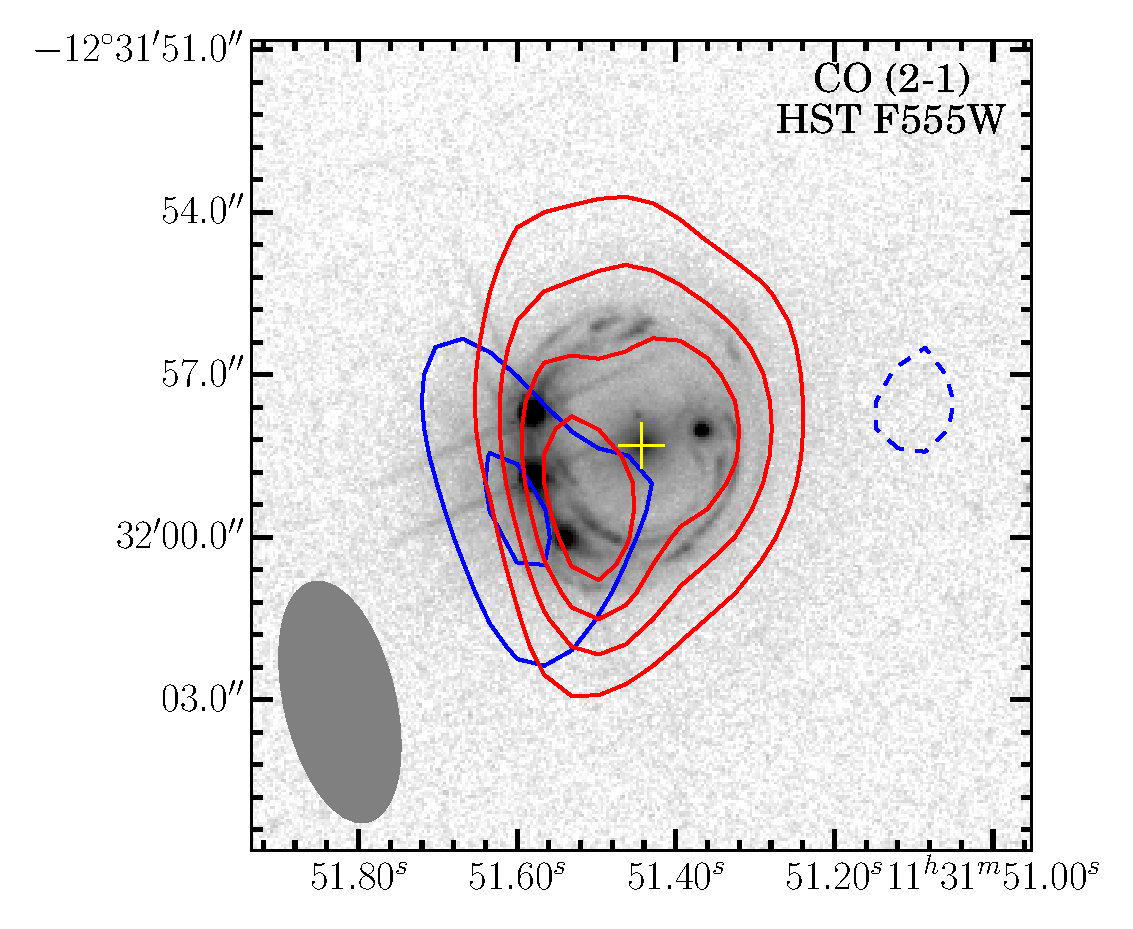
\includegraphics[trim=3 5 0 0, clip, width=0.23\textwidth]{../Figures/F555W_REDBLUE.eps}
\caption{Left: an overlay of the velocity-integrated \bco emission on the {\it HST} $V$--band (F555W)
image. Right: contours are color-coded to represent the red and blue wings of the emission.
The contours start at 3$\sigma$ and increment at steps of
$\pm$3$\sigma$, where $\sigma$\,=\,0.3 mJy beam\pmOne. The crosses denote the
location of the foreground galaxy at $z$\,=\,0.295.
\label{fig:CO21mom}}
\end{figure}

The emission of the red component coincides with the Einstein Ring seen in the
optical image, with most of its apparent flux originating from the lensed arc
in the southeast, whereas the blue component is predominately coming from
solely the lensed arc shown in \Fig{CO21mom}. To illustrate this, we show the
channel maps of 21.5\,\kms width and spatial spectra of 1\farcs5 resolution in
\Fig{chanmap} and \Fig{spatialSpec}, respectively. The figures
show that emission
is present to the west, peaking toward the lensing arc (black crosses in
\Fig{chanmap}) in the red wing, and shifts to the east with decreasing velocity
(blue wing).
This indicates extended emission in the source plane, where
emission from different kinematic components is separated by different amounts
relative to the caustics, leading to the observed asymmetric
line profile. A detailed analysis on differential lensing of \bco is presented
in \Sec{differential}, where we present our lens model.

\begin{figure*}[!htbp]
\centering
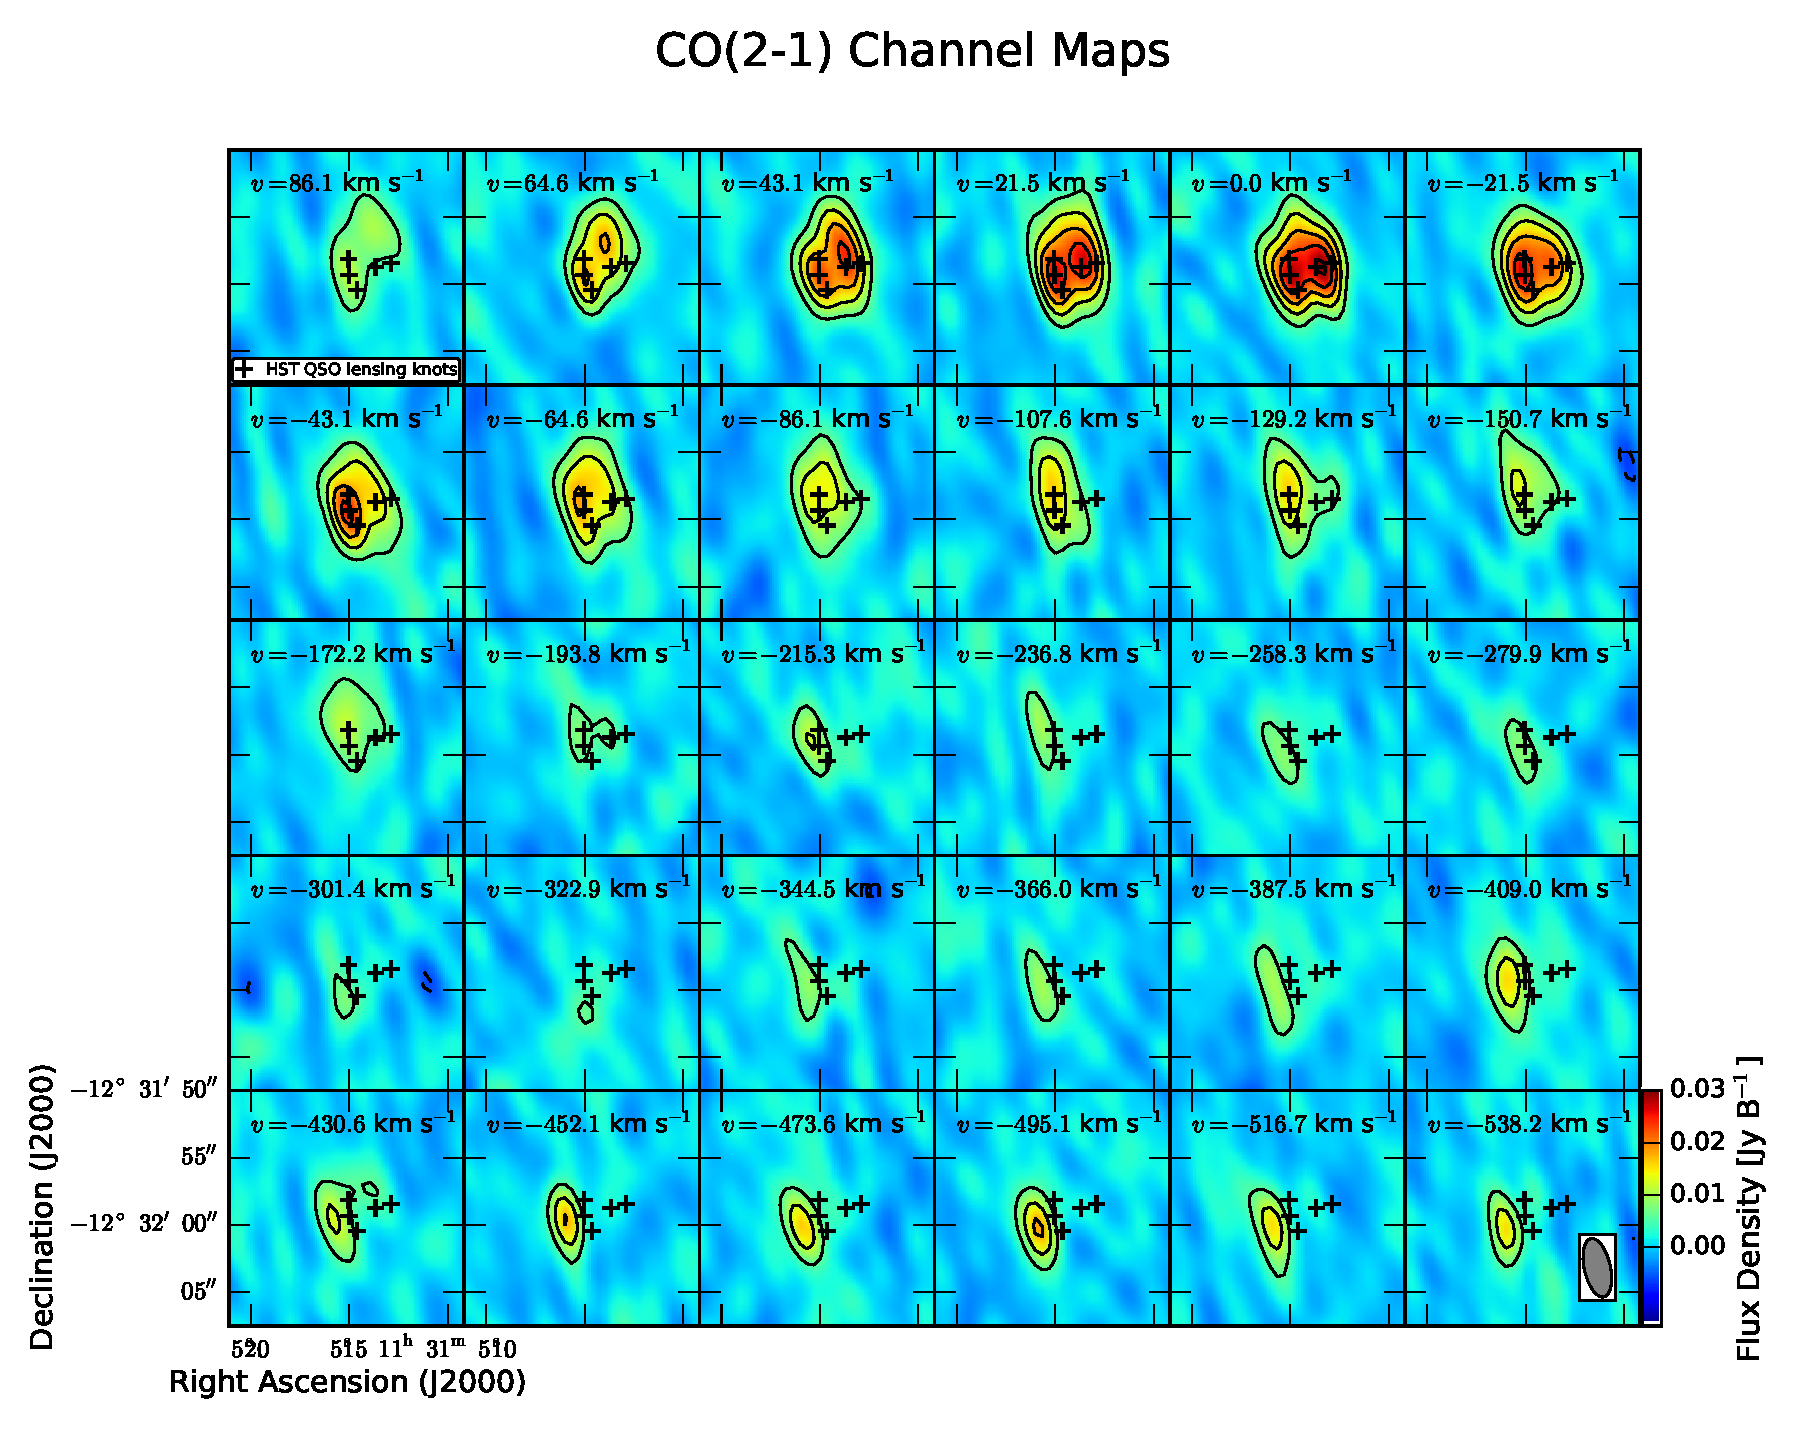
\includegraphics[width=1.0\textwidth]{../Figures/co_channel_maps.eps}
\caption{
Channel maps of PdBI \bco toward RXJ1131 in 21.5\,\kms resolution.
Black crosses indicate the position of the lensed knots (AGN emission,
which correspond to components ABCD in C06). The central white-filled
star indicates the position of the foreground lensing galaxy (component G
in C06). Contours start and increment at steps of
$\pm$3$\sigma$. The beam is denoted in the bottom right panel. \label{fig:chanmap}}
\end{figure*}

\begin{figure*}[!htbp]
\centering
\includegraphics[width=0.9\textwidth]{../Figures/spatialSpec_offsetShifted.eps}
\caption{
\bco spectrum as a function of position, binned by 3 pixels in each
direction (1\farcs5).
The spectra map covers an extent of $\sim$10"$\times$10"
centering on the pixel that corresponds to the lensing galaxy.
Spatial offset in arcsec is denoted in top left corner of each panel.
The velocity and flux density scales are denoted in the top right panel.
\label{fig:spatialSpec}}
\end{figure*}

We also place an upper limit on \rot[HNC]{2}{1} line emission
in the foreground galaxy at $z\sim$0.295.
Assuming a typical line width of 300\,\kms, this corresponds to a 3$\sigma$
limit of 0.35\,mJy\,\kms\,beam\pmOne.

\subsection{Origin of the \bco Emission} \label{sec:origin} %DONE
Evidently, the CO emission is co-spatial with the lensed optical emission in
the background AGN host galaxy.
The question is then whether the optically
faint companion also contributes to the CO flux and thus contains a
non-negligible amount of molecular gas.
Indeed, based on our lens model presented in \Sec{lensmodel}, we find it
highly likely that part of the CO emission originates from
the companion. We thus classify RXJ1131 as a ``wet-wet'' merger.
However, we cannot quantify this with a mass ratio given the
spatial resolution, nor can we rule out the possibility that
the ``companion'' is instead a gas component/tidal feature ripped out
from previous interaction.
In the subsequent sections, we will interpret
the this additional source component as gas emission
in a nearby galaxy (i.e. a ``wet-wet'' merger), as suggested by previous studies of RXJ1131 (C06, B08).

\subsection{\bco Kinematics} % DONE
A clear velocity gradient and a high
velocity dispersion ($\gtrsim$400\,\kms) near the central region
is seen in \Fig{CO21highO}. While beam smearing is inevitably the
dominant factor in the observed velocity dispersion
at the spatial resolution of this data, the exceedingly
high velocity dispersion may hint
at potential perturbations from the AGN, or internal turbulence due to
interactions with the companion, and/or instability due to the large gas
content. A velocity gradient across the source plane in \Fig{model} is also
found in our lens model. This further supports the idea of a
kinematically-ordered galaxy, but its emission has been lensed differentially.
In this scenario, RXJ1131 is a disrupted disk galaxy hosting an optically
bright quasar and is in the process of merging.
We will defer the discussion of its implications to \Sec{dynamics},
where we analyze the dynamics of the system in the source plane.

\begin{figure}[!htbp]
\centering
\includegraphics[width=0.45\textwidth]{../Figures/CO_highOmom_CLIP5sigma}
\caption{
Contours for the first (left) and second (right) moment maps are shown in steps of
50 \kms, and 100 \kms, respectively. The beam (native resolution) is shown in the right panel.
\label{fig:CO21highO}}
\end{figure}


\subsection{\cco Emission} % DONE
We detect resolved \cco line emission toward RXJ1131. The spectrum is shown in
\Fig{co32spec}, which seems to have a double-peak profile.
This is expected if RXJ1131 is truly a disk galaxy (see previous
sections). The high phase noise in the calibration leads to a low SNR
detection. We thus estimate the line intensity to be
35.7\,$\pm$\,21.9 Jy\,\kms by summing up fluxes over the FWZI
linewidth used to infer \bco line intensity ($\sim$700 \kms).

\begin{figure}[!Htbp]
\centering
\includegraphics[width=0.455\textwidth]{../Figures/coOverlay.eps}
\caption{CARMA \cco line profile (solid) without continuum subtraction is
over-plotted on the continuum-subtracted PdBI \bco line profile (dashed).
The velocity scale is with respect to $z$=0.6537, which corresponds to the
dynamical center of the \bco line. The spectral resolution for \cco and \bco
is 35.8 \kms and 21.5 \kms, respectively.
 \label{fig:co32spec}}
\end{figure}

Assuming the spatial extents between \bco and \cco are similar and therefore
a negligible differential lensing effect, the line intensities
correspond to a brightness temperature ratio of
$r_{\rm 32}$\,=\,T$_{\small \cco}$$/$T$_{\small \bco}$\,=\,0.66\,$\pm$\,0.41.

\subsection{Continuum Emission} %DONE
No 1.5\,mm continuum emission is detected at the position of \cco
down to a 3$\sigma$ limit of 2.49\,mJy beam\pmOne.
This is consistent with the spectrum shown in \Fig{co32spec}.

We detect PdBI 2\,mm continuum in \Fig{cont}. The integrated flux density is
1.2\pmm0.2 mJy, with a peak flux
$S_\nu$\,=\,800\pmm88\,$\mu$Jy\,beam\pmOne
centering on the lensing galaxy. Slightly extended emission is also detected
along the lensed arc. This suggests that the detected emission comes from
both the foreground galaxy and the background galaxy and that the
emission is marginally resolved along its major axis.
We subtract a point source model in $uv$-plane to remove the unresolved
emission toward the foreground galaxy. The peak flux (0.39\,$\pm$\,0.08\,mJy)
in the residual map coincides with the lensed arc, and is consistent with
the difference between the integrated and the peak flux in the
original continuum map ($\sim$0.4 mJy). We therefore adopt
$S_\nu$ = 0.39\pmm0.08 mJy as the 2\,mm continuum emission toward
the background galaxy.

\begin{figure}[!htbp]
%\centering
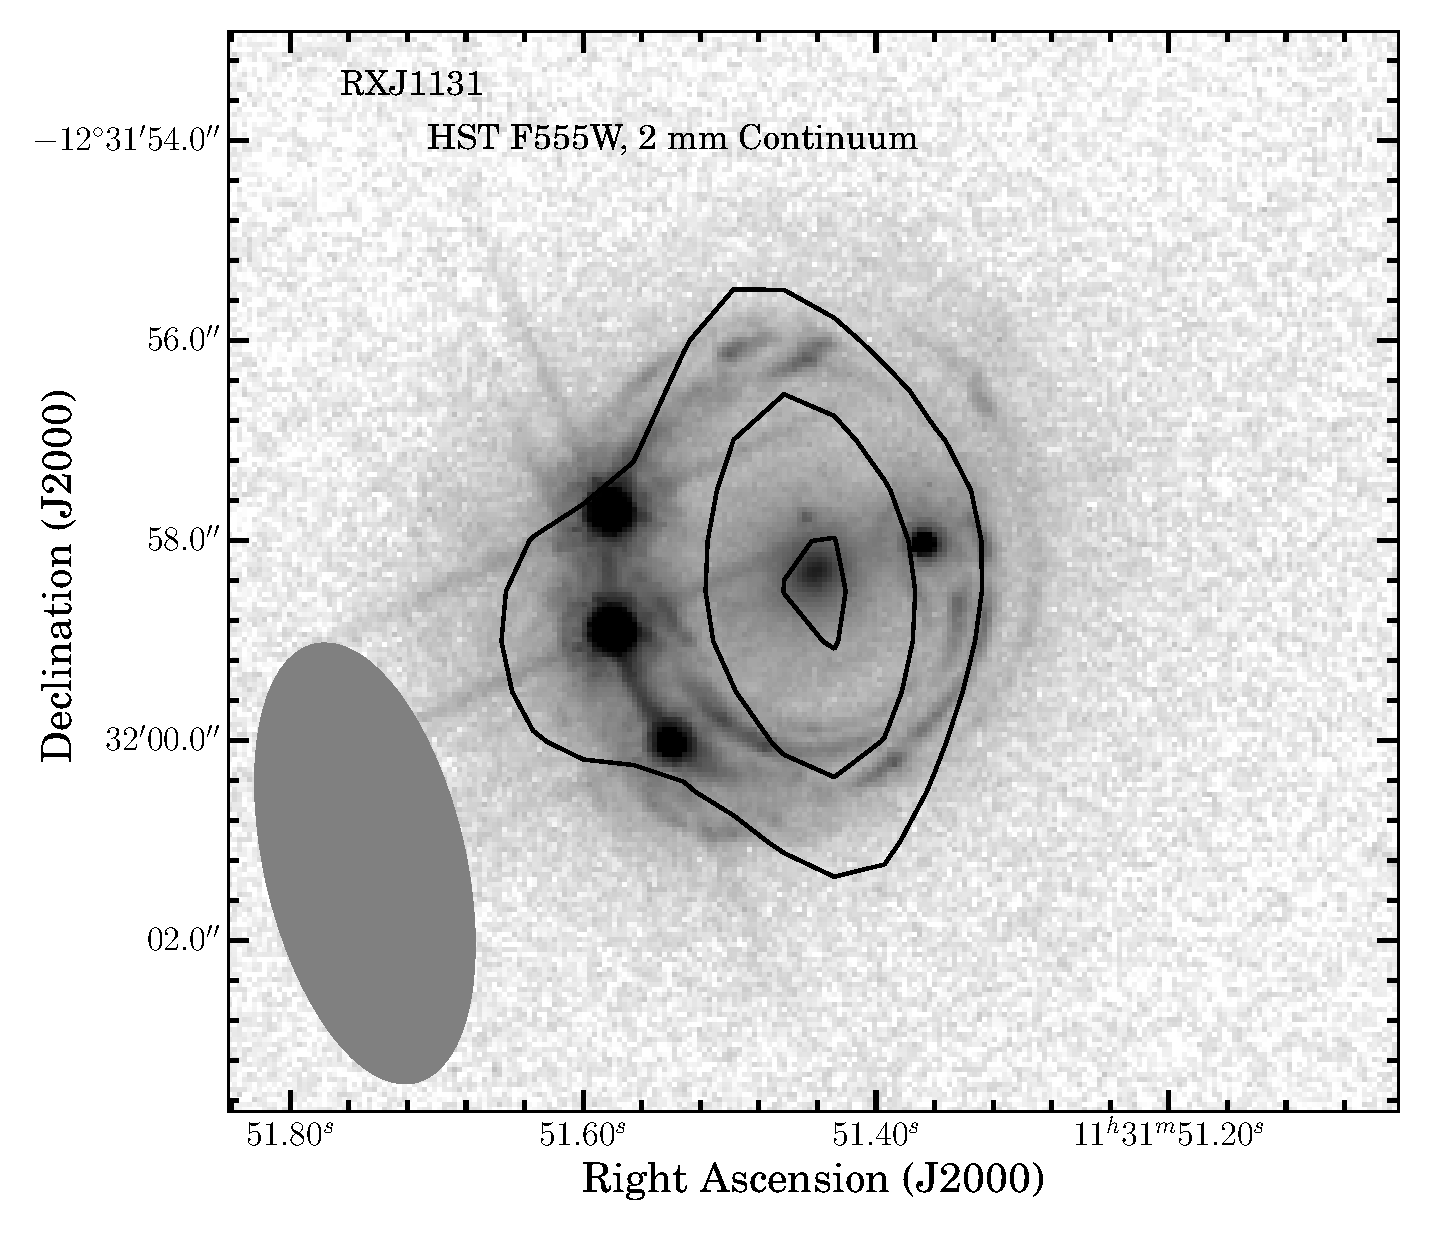
\includegraphics[trim=12 27 0 1, clip, width=0.475\textwidth]{../Figures/F555W_ContPdBI.eps}
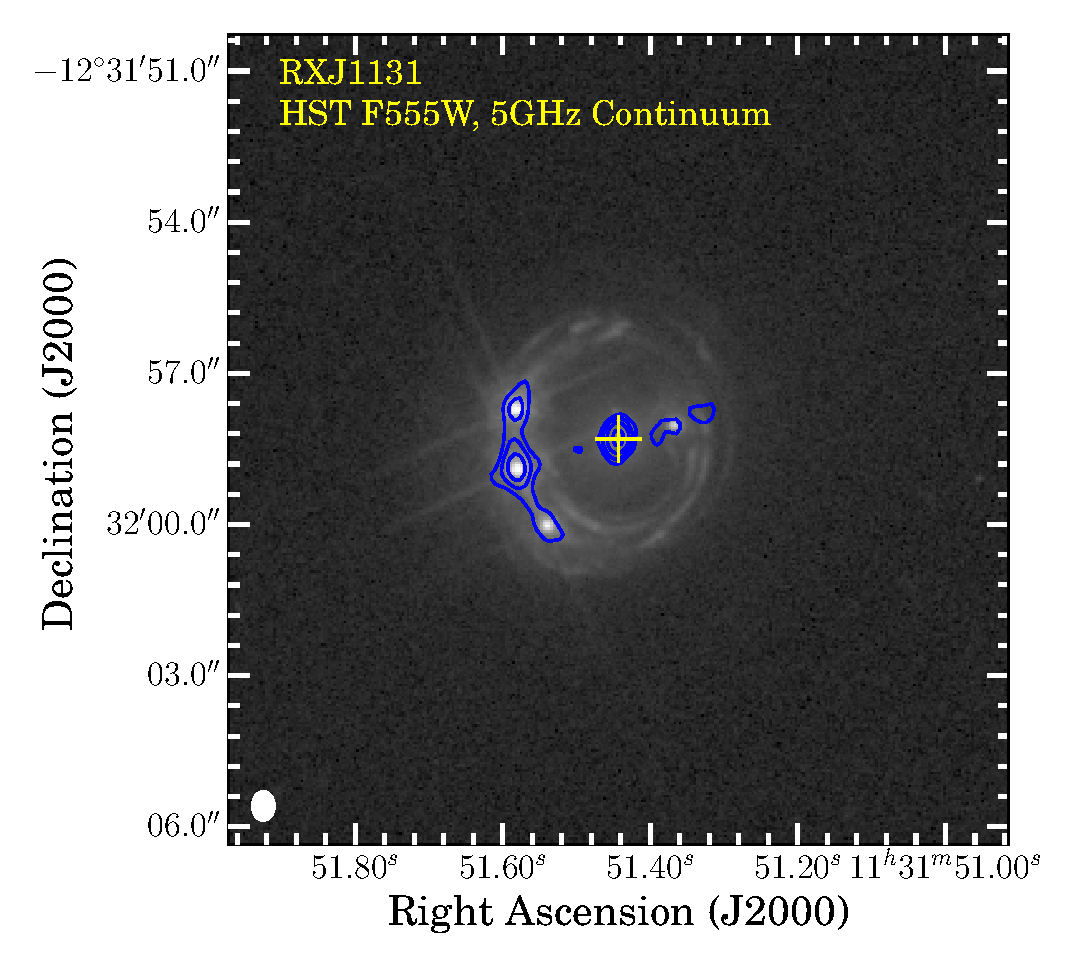
\includegraphics[trim=13 5 0 0, clip, width=0.475\textwidth]{../Figures/F555W_ContVLA.eps}
\caption{Top: an overlay of the 2\,mm continuum emission on the optical image.
Bottom: VLA 5\,GHz continuum emission is overlaid on the optical image.
Contours in both images start and increment at steps of
$\pm$3$\sigma$, where $\sigma_{\rm 2mm}$\,=\,0.082 mJy beam\pmOne and
$\sigma_{\rm 5GHz}$\,=\,13 $\mu$Jy beam\pmOne in the left and right panel, respectively.
The central crosses indicate the centroid of the foreground galaxy,
as detected in the optical image. The synthesis beams are shown in the bottom left corner of each panel.
\label{fig:cont}}\vspace{0.51em}
\end{figure}

The VLA C-band continuum image in \Fig{cont} shows resolved emission from the
jets and core of the foreground elliptical galaxy
as well as emission toward the background quasar.
Multiple peaks are seen along the arc and their centroids
coincide with the optical emission from the quasar.
We extract the flux densities for the arc and the core in \Tab{photometry}.
We find a spectral index of $\alpha^{\rm 2mm}_{\rm 6cm}$\,=\,$-$0.024
for the foreground
galaxy and $\alpha^{\rm 2mm}_{\rm 6cm}$\,=\,$-$0.345
for the background galaxy by fitting a
power-law (S$_\nu \propto \nu^{\alpha}$) to the continuum emission at
5\,GHz and 2\,mm.

\subsection{Photometry} \label{sec:photometry} %DONE
We compile \mir (MIR) to \fir broadband photometry from various
catalogs available on the NASA/IPAC Infrared Science
Archive (IRSA) in \Tab{photometry} with aperture corrections
when warranted. These data were obtained from
the Two Micron All Sky Survey (2MASS; \citealt{Skrutskie06a}),
the Wide-field Infrared Survey Explorer ({\it WISE}; \citealt{Wright10a}),
the {\it Infrared Astronomical Satellite}
({\it IRAS};\citealt{Neugebauer84a}), and
the Multiband Imaging Photometer (MIPS; \citealt{Rieke04a}) and
Mid-infrared Infrared Array Camera (IRAC; \citealt{Fazio04a}) on
the \spitzer.
We retrieve PBCD (level 2) {\it Spitzer}/IRAC images from the
Spitzer Heritage Archive and perform aperture photometry on
the channel 1 image to extract the flux density at 3.6\,$\mu$m
since it is not available from the IRSA archive.

The emission in the IRAC images is slightly extended. We thus use the
{\it HST} image ($\sim$0\farcs07 resolution) to determine
origins of their centroids, all of which are found to be
centered at the position corresponding to the lensed emission from the
background galaxy. To recover the diffuse background emission, we subtract a
point source model centered on the lensing galaxy, using the average
FWHM found by fitting a Gaussian profile to several field stars
with the \ncode{imexam} routine of IRAF.
We perform aperture photometry on the residual image
to obtain decomposed flux measurements from the background galaxy.
The photometry for the foreground galaxy is then obtained
by subtracting the background emission from the
observed total flux. The resulting photometry in
\Tab{photometry} are obtained after performing an aperture correction
described in the IRAC Instrument Handbook\footnote{http://irsa.ipac.caltech.edu/data/SPITZER/docs/irac/iracinstrumenthandbook/} to
correct for the fact that the imaging was calibrated
using a 12" aperture, which is larger than the aperture (5\farcs8) we used to
perform aperture photometry.

We fit a power-law spectrum to the
decomposed IRAC photometry to disentangle the observed total flux
at MIPS 24\,$\micron$ into the foreground and
background galaxies. We find a spectral index of $\alpha\sim-$1.8 and
$\alpha\sim-0.85$ for the lensing galaxy and RXJ1131, respectively.
This is consistent with the mean 3.6\,$-$\,8\,$\micron$
spectral slope of
$\alpha$\,=\,$-$1.07\,$\pm$\,0.53 found for unobscured AGN
\citep{Stern05a}. An extrapolation of the fit to 24$\micron$
yields 33.96\,$\pm$\,0.01\,mJy and 25.19\,$\pm$\,0.03\,mJy
for the foreground galaxy and RXJ1131, respectively.
We note that the IRAC photometry includes
emission from old stellar population and is prone to
dust extinction. Hence, the decomposed fluxes are only
our best estimate of the warm dust emission.
We incorporate the decomposed 24$\micron$ point in our
SED fitting to provide some constraints on
the Wien tail beyond the dust peak
of the spectral energy distribution (SED) of RXJ1131.
Details of the SED modeling is presented in \Sec{SED}.

Extraction of the {\it Herschel}/SPIRE photometry was
carried out using \ncode{sussextractor} within the Herschel Interactive
Processing Environment (HIPE; \citealt{Ott10a})
on Level 2 maps obtained from the Herschel Science Archive.
These maps were processed by the SPIRE pipeline
version 13.0 within HIPE. The \ncode{sussextractor} task estimates
the flux density from an image convolved with a kernel
derived from the SPIRE beam. The flux density
measured by \ncode{sussextractor} is additionally confirmed
using the Timeline Fitter, which performs photometry
by fitting a 2D elliptical Gaussian to the Level 1 data at the
source position given by the output of \ncode{sussextractor}.

\begin{deluxetable}{lccc}[tbpH]
\tabletypesize{\scriptsize}
\tablecolumns{4}
\tablecaption{Photometry data}
\tablehead{\colhead{Wavelength } & \colhead{Frequency } & \colhead{Flux Density } & \colhead{Instrument}\\ \colhead{micron} & \colhead{GHz} & \colhead{mJy} & \colhead{ }}
\startdata
0.555 & 540167.0 & 0.056 $\pm$ 0.006 & HST-ACS/V-Band(L) \\
0.555 & 540167.0 & 0.009 $\pm$ 0.0041 & HST-ACS/V-Band(H) \\
0.814 & 368295.0 & 0.238 $\pm$ 0.013 & HST-ACS/I-Band(L) \\
0.814 & 368295.0 & 0.041 $\pm$ 0.0054 & HST-ACS/I-Band(H) \\
1.25 & 239834.0 & 1.009 $\pm$ 0.09 & 2MASS/J-Band \\
1.6 & 187370.0 & 0.539 $\pm$ 0.041 & HST-NICMOS(NIC2)/H-Band(L) \\
1.6 & 187370.0 & 0.133 $\pm$ 0.004 & HST-NICMOS(NIC2)/H-Band(H) \\
1.65 & 181692.0 & 1.448 $\pm$ 0.12 & 2MASS/H-Band \\
2.17 & 138153.0 & 2.064 $\pm$ 0.16 & 2MASS/Ks-Band \\
3.4 & 88174.2 & 7.027 $\pm$ 0.14 & WISE/W1 \\
3.6 & 83275.7 & 5.618 $\pm$ 0.0021 & Spitzer/IRAC(Extracted) \\
3.6 & 83275.7 & 5.034 $\pm$ 0.0021 & Spitzer/IRAC(Host) \\
3.6 & 83275.7 & 0.585 $\pm$ 0.003 & Spitzer/IRAC(Archive-Host) \\
4.5 & 66620.5 & 7.803 $\pm$ 0.0021 & Spitzer/IRAC(Archive) \\
4.5 & 66620.5 & 6.009 $\pm$ 0.0017 & Spitzer/IRAC(Host) \\
4.5 & 66620.5 & 1.794 $\pm$ 0.0027 & Spitzer/IRAC(Archive-Host) \\
4.6 & 65172.3 & 8.872 $\pm$ 0.16 & WISE/W2 \\
5.8 & 51688.4 & 10.720 $\pm$ 0.0051 & Spitzer/IRAC(Archive) \\
5.8 & 51688.4 & 7.557 $\pm$ 0.003 & Spitzer/IRAC(Host) \\
5.8 & 51688.4 & 3.163 $\pm$ 0.0059 & Spitzer/IRAC(Archive-Host) \\
8.0 & 37474.1 & 14.470 $\pm$ 0.0041 & Spitzer/IRAC(Archive) \\
8.0 & 37474.1 & 9.881 $\pm$ 0.0039 & Spitzer/IRAC(Host) \\
8.0 & 37474.1 & 4.589 $\pm$ 0.0057 & Spitzer/IRAC(Archive-Host) \\
12.0 & 24982.7 & 21.960 $\pm$ 0.42 & WISE/W3 \\
12.0 & 24982.7 & 400.000 $\pm$ \nodata & IRAS \\
22.0 & 13626.9 & 55.110 $\pm$ 1.9 & WISE/W4 \\
24.0 & 12491.4 & 47.180 $\pm$ 0.026 & Spitzer/MIPS \\
25.0 & 11991.7 & 500.000 $\pm$ \nodata & IRAS \\
60.0 & 4996.54 & 600.000 $\pm$ \nodata & IRAS \\
100.0 & 2997.92 & 1000.000 $\pm$ \nodata & IRAS \\
250.0 & 1199.17 & 289.427 $\pm$ 9.6 & Herschel/SPIRE \\
350.0 & 856.55 & 168.229 $\pm$ 8.6 & Herschel/SPIRE \\
500.0 & 599.585 & 56.782 $\pm$ 8.8 & Herschel/SPIRE \\
1387.93 & 216.0 & 2.492 $\pm$ \nodata & CARMA \\
2152.82 & 139.256 & 1.230 $\pm$ 0.22 & PdBI-integrated \\
2152.82 & 139.256 & 0.799 $\pm$ 0.082 & PdBI-peak \\
2152.82 & 139.256 & 0.400 $\pm$ 0.082 & PdBI-removedFG \\
61414.0 & 4.8815 & 1.273 $\pm$ 0.042 & VLA/Cband-arc \\
61414.0 & 4.8815 & 0.866 $\pm$ 0.027 & VLA/Cband-core
\enddata
\label{tab:BLAH}
\tablecomments{blah}
 %TablenotegoesBetween 
\tablerefs{blah}
\end{deluxetable}


%--------------------------------------------------------------------------
%                                Analysis
%--------------------------------------------------------------------------
\section{Analysis} \label{sec:anal}
\subsection{Lens modeling} \label{sec:lensmodel} %DONE
At the angular resolution of the \bco data, the images are resolved
but not within the multiply lensed emission (i.e., sub-optimal for
performing lens modeling). Nevertheless, the high spectral
resolution of this data provides dynamical information on
spatial scales smaller than the beam (see \Fig{CO21highO}).
Hence, with the high SNR, we reconstruct the intrinsic gas
dynamics by carrying out a parametric lens modeling over different
channel slices of the interferometric data using our lensing code
\uvmcmcfit (\citealt{uvmcmcfit15a}; see \citealt{Bussmann15a} for details of
the code). Model of each slice in \Fig{model} thus provides
properties on the intrinsic kinematics. The slices
are obtained by binning the data over the full linewidth
$\sim$700\,\kms by five channels,
that is, into seven slices, to increase the SNR.

The lens mass distribution is modeled using a singular isothermal
ellipsoid (SIE) profile, which is described by five free parameters: the
positional offset in R.A. and Dec. relative to an arbitrary chosen
fixed coordinate in the image, the Einstein Radius, the axial ratio, and the
position angle. We use the VLA radio continuum emission toward
the foreground galaxy to initialize the positional offset. We impose a
uniform prior $\pm$0\farcs05 in both $\Delta$R.A. and $\Delta$Dec.,
motivated by the astrometry uncertainties in the VLA image as well as
the uncertainties provided by previous SIE lens model (C06).
We initialize the Einstein Radius based on the model parameters reported by C06
and impose a uniform prior using $\pm$3$\sigma$ of their uncertainties.
The sources are modeled using elliptical Gaussian profiles, which are
parameterized by six free parameters: the positional offset in R.A.
and Dec. relative to the lens, the intrinsic flux density, the effective
radius, the axial ratio, and the position angle. The position of each source
is allowed to vary between $\pm$1\farcs5 (i.e., within the Einstein Radius)
and the effective radius is allowed to vary from 0\farcs01$-$2$^{\prime\prime}$.

Our code uses an Markov Chain Monte Carlo (MCMC) approach to sample the
posterior probability distribution function (PDF).
In each model, we require a target acceptance rate of $\sim$0.25$-$0.5
and check for chain convergence by inspecting trace plots
and requiring the samples are beyond at least an autocorrelation time.
We thus employ $\sim$50,000 samples as the initial ``burn-in'' phase
to stabilize the Markov chains (which we then discard) and
use the final $\sim$5,000 steps, sampled by 128 walkers, to identify
the posterior. Here, we
identify the best-fit model and the quoted uncertainties using the
median and the 68\% confidence intervals in the marginal PDFs.
\begin{deluxetable*}{lcc}[!htbp]
\tabletypesize{\scriptsize}
\tablecolumns{3}
\tablecaption{Lens parameters from preliminary models}
\tablehead{
\multicolumn{2}{c}{Parameters} &
\colhead{Median values} % weighted-mean of median of each
}
\startdata
Offset in RA    & (\arcsec)   &  0.004$\pm$0.027\\
Offset in Dec    & (\arcsec)   & 0.003$\pm$0.027\\
Axial Ratio      &             & 0.56$\pm$0.16\\
Position Angle   & (deg)       & 103$\pm$22\\
Einstein Radius  & (\arcsec)   & 1.833$\pm$0.002\\
\enddata
\label{tab:lens}
\tablecomments{ Parameters describing the foreground lens are
obtained based on the preliminary models (see text for details).
All angular offsets are with respect to
$\alpha$\,=\,11$^{\rm h}$31$^{\rm m}$51\fs44,
$\delta$\,=\,-12\degr31\arcmin58\farcs3 (J2000).
The corresponding masses
within the Einstein radii is $M(\theta$\,\,$<$\,\,$\theta_\textrm{E})$\,=\,(7.47\,$\pm$\,0.02)\,$\times$\,10$^{11}$\,\,\Msun.}
\end{deluxetable*}


We first obtain a preliminary lens model for each channel slice independently,
where their lens parameters are allowed to vary and are initialized according
to the aforementioned way. We obtain the final model
by repeating the modeling over each slice but fixing their lens parameters
according to the overall median in the preliminary models,
as listed in \Tab{lens}.
This ensures that all models share the same lens profile.
The magnification factors in \Tab{model} are determined by taking the ratio
between the image plane flux and the source plane flux of each model.

Our model parameters in \Tab{lens}, describing
the mass distribution of the lensing galaxy, are consistent (within the uncertainties)
with that of the SIE model presented by C06. We find a mass of
$M(\theta$\,\,$<$\,\,$\theta_\textrm{E})$\,=\,(7.47\,$\pm$\,0.02)\,$\times$\,10$^{11}$\,\Msun
within the Einstein radius.

\subsubsection{Interpretation and Caveats} \label{sec:caveat} %DONE
The reconstructed source locations in \Fig{model} demonstrate
an intrinsic velocity gradient across the source plane, which is
indicative of a disk-like galaxy.
Additional support to the disk conjecture %conjecture of a disk morphology
can be found in the double-horned line profile (\Fig{CO21spec})
and the observed (image plane) velocity field (\Fig{CO21highO}). Furthermore,
C06 also find that the reconstructed source plane emission in optical-NIR
is best-reproduced using a $n$\,=\,1 Sersic profile.
Our interpretation therefore tends in favor of a disk morphology for RXJ1131.

% the companion
One other interesting result from our lens model is that a better fit is
found for the red-most channel if we add a second source component (see
top left panel in \Fig{model}). This is consistent with previous results
reported by \citet{Brewer08a}, who find an optically faint companion
(component F in their paper) $\sim$2.4\,kpc away from the AGN host galaxy,
and C06, who find evidence for an interacting galaxy near RXJ1131.
Spatially, the red velocity component of the CO also coincides with this
component F. While we cannot quantify the type of
merger (major v.s. minor) with a mass ratio given the
spatial resolution, the symmetric velocity gradient retained under
such close separation between the two lean support
to the idea of a minor merger.
% For major mergers, two galaxy mass centers separated on the same scale as the
% gas disk (4 kpc or more), the gas dynamics would be strongly perturbed and
% would deviate substantially from that of a simple disk.
% In a minor merger (a mass ratio of more than 3:1) the more massive galaxy, including its gas distribution, can retain a significant angular momentum and resemble a rotating disk.

The spatial resolution of the data in hand
is a few arcsec, which implies that despite the high SNR and spectral
resolution, this data is insufficient to constrain the
intrinsic sizes of the lensed galaxies, and thus the magnification
factors may be under-predicted.
% magnification factor is underpredicted, see Bussmann15

\begin{figure*}[tbph]
\centering
\begin{tabular}{c}
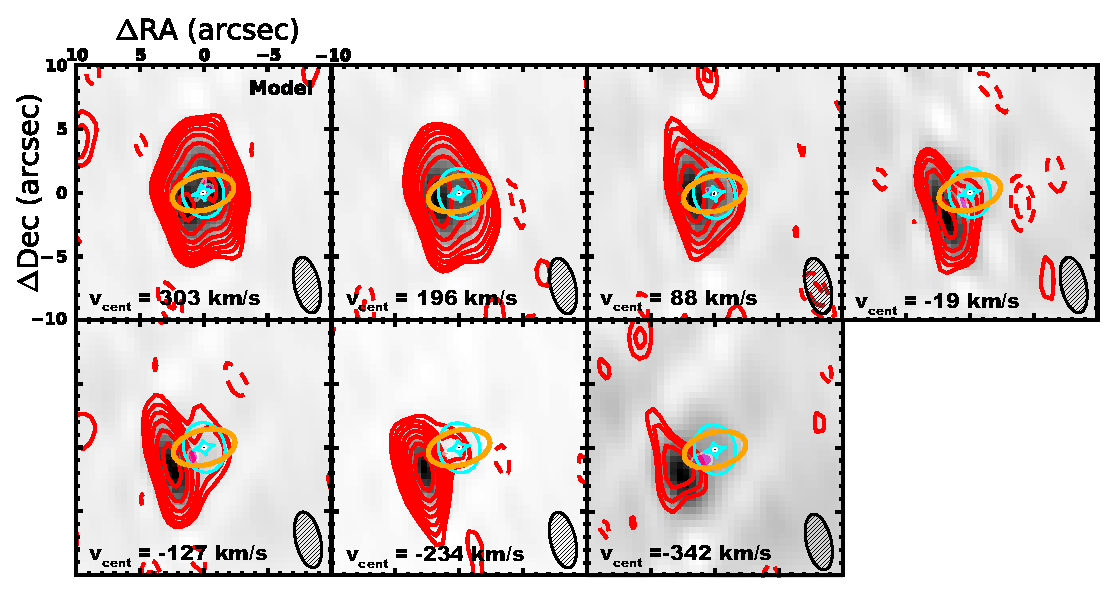
\includegraphics[trim=0 0 0 0, clip, width=1.0\textwidth]{../Figures/PostageStampModel.eps} \\
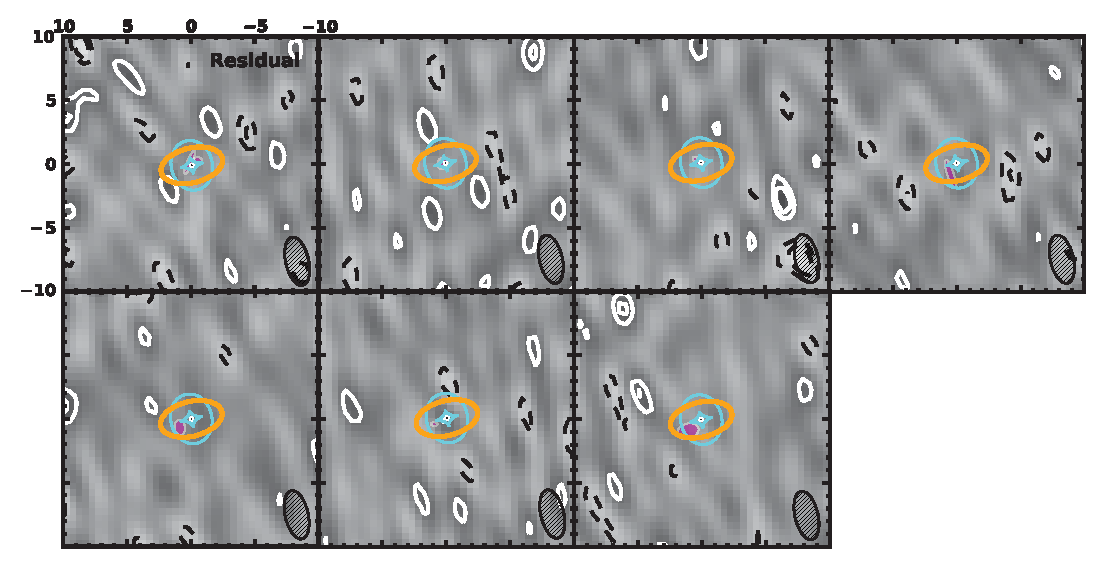
\includegraphics[width=0.98\textwidth]{../Figures/PostageStampResiduals.eps}
\end{tabular}
\caption{Each panel corresponds to a lens model of RXJ1131 performed over a
channel slice $\sim$100\,\kms of the \bco data. Top: channel maps of the
PdBI \bco emission (red) overlaid on our best-fit lens models (grayscale).
The location of the foreground lensing galaxy is indicated by a black dot and
its critical curve is traced by the orange solid line. The locations and
morphologies (half-light radii) of the reconstructed sources are
represented by magenta ellipses (see text in \Sec{caveat} for caveats).
The caustic curves are represented as cyan lines. The beam of the
PdBI observations is shown in the bottom right corner of each panel.
Bottom: residual images of the best-fit models, obtained by
taking the Fourier transform after subtracting the best-fit model from the
data in the $uv$-domain. Contours start
at $\pm$3$\sigma$ and increment at steps of 3$\times$2$^n\sigma$,
where $n$ is a positive integer.
\label{fig:model}}
\end{figure*}

\subsubsection{Differential Lensing} \label{sec:differential} %DONE
\begin{deluxetable}{lcc}[!htbp]
\tabletypesize{\scriptsize}
\tablecolumns{3}
\tablecaption{Magnification factors of various kinematic components in \bco}
\tablehead{
\colhead{Velocity Range(\kms)} & % see 22May16/intensity30Apr16.spec; or channel map in paper
\colhead{Source 1 $\mu_{\rm L}$} &
\colhead{Source 2 $\mu_{\rm L}$}
}
\startdata
$-$366\,$-$\,$-$258 & 3.1 $\pm$ 0.9 & \\ [0.5ex]
$-$237\,$-$\,$-$151 & 4.3 $\pm$ 2.4 & \\ [0.5ex]
$-$129\,$-$\,$-$43  & 4.2 $\pm$ 0.6 & \\ [0.5ex]
$-$21.5\,$-$\,65    & 4.1 $\pm$ 0.9 & \\ [0.5ex]
86\,$-$\,172        & 8.7 $\pm$ 2.0 & \\ [0.5ex]
194\,$-$\,280       & 7.6 $\pm$ 1.6 & \\ [0.5ex]
301\,$-$\,388       & 7.2 $\pm$ 5.6 & 6.7 $\pm$ 2.5 \\ [0.5ex]
weighted average & 4.4 & \\ [0.5ex]
median & 5.5 &
\enddata
\label{tab:model}
\tablecomments{Velocity is taken from the center of each (native) channel
without any binning. Each row corresponds to a channel slice used for
lens modeling. Source 1 is RXJ1131 and source 2 is its companion. See text for details. }
\end{deluxetable}

Previous lens models of RXJ1131 find evidence for
differential lensing across {\it HST}
$H$-, $V$-, and $I$-band (C06), where the
magnification factor ranges from 10.9 to 7.8. C06 attribute
the decrease toward the IR regime is caused by the more extended
IR emission. The highly asymmetric \bco line profile suggests that
differential lensing is also non-negligible for CO, where the redshifted
emission is apparently much brighter than that in the
blueshifted part, consistent
with the source positions relative to the caustics in \Fig{model}.
The red wing emission mainly originates near the cusp
in the caustic, whereas the blue wing emission is located beyond the caustics.
The magnification factor for CO ranges from 8.7 to 3.1 (\Tab{model}).

\subsection{\bco Dynamical modeling} \label{sec:dynamics} %DONE
Assuming the velocities of the respective channels used in the
lens modeling correspond to solely the tangential component of the
true velocity vector of a rotating disk (i.e., along the major axis),
we extract a one dimensional PV diagram in \Fig{PV}
by slicing across their source plane positions (PA: 121\degr).

We then attempt to characterize the molecular gas kinematics using an
empirically-motivated disk model \citep[\eg][]{Courteau97a,Puech08a,Miller11a}:
\begin{equation}
V = V_0 + \frac{2}{\pi} V_{a} \arctan(\frac{R}{R_{t}}),
\end{equation}
where $V$ is the observed velocity, $V_0$ is the velocity at dynamical center,
$V_{a}$ is the asymptotic velocity, and $R_{t}$ is the ``turnover''
radius at which the rotation curve becomes flat.
We perform non-linear least square fitting using an orthogonal distance
regression to find the best-fit parameters,
taking into account the uncertainties in both velocity (channel width) and
distance offset. We also place an upper limit on $R_{t}$\,$<$15 kpc
to keep this parameter physical \citep[\eg][]{Puech08a,Miller11a}.
The parameter uncertainties are inferred based on Monte Carlo simulation
of 500 iterations, where the input parameters are perturbed
according to random Gaussian distributions of sigmas
corresponding to their uncertainties.
Using this model, we find $V_{a}$\,=\,975\,$\pm$\,387 \kms,
$R_{t}$\,=\,10.6\,$\pm$\,5.7\,kpc, and $V_0$\,=\,28\,$\pm$\,40 \kms.
However, since emission is not resolved along the flat regime
of the rotation curve, the asymptotic velocity is poorly constrained and
the ``turnover'' radius is at most a lower limit.
In particular, $V_{a}$ and $R_{t}$ are highly correlated with a
Pearson coefficient $R$\,=\,0.998, and 0.027 between $V_{a}$ and $V_0$.

\begin{figure}[!htbp]
\centering
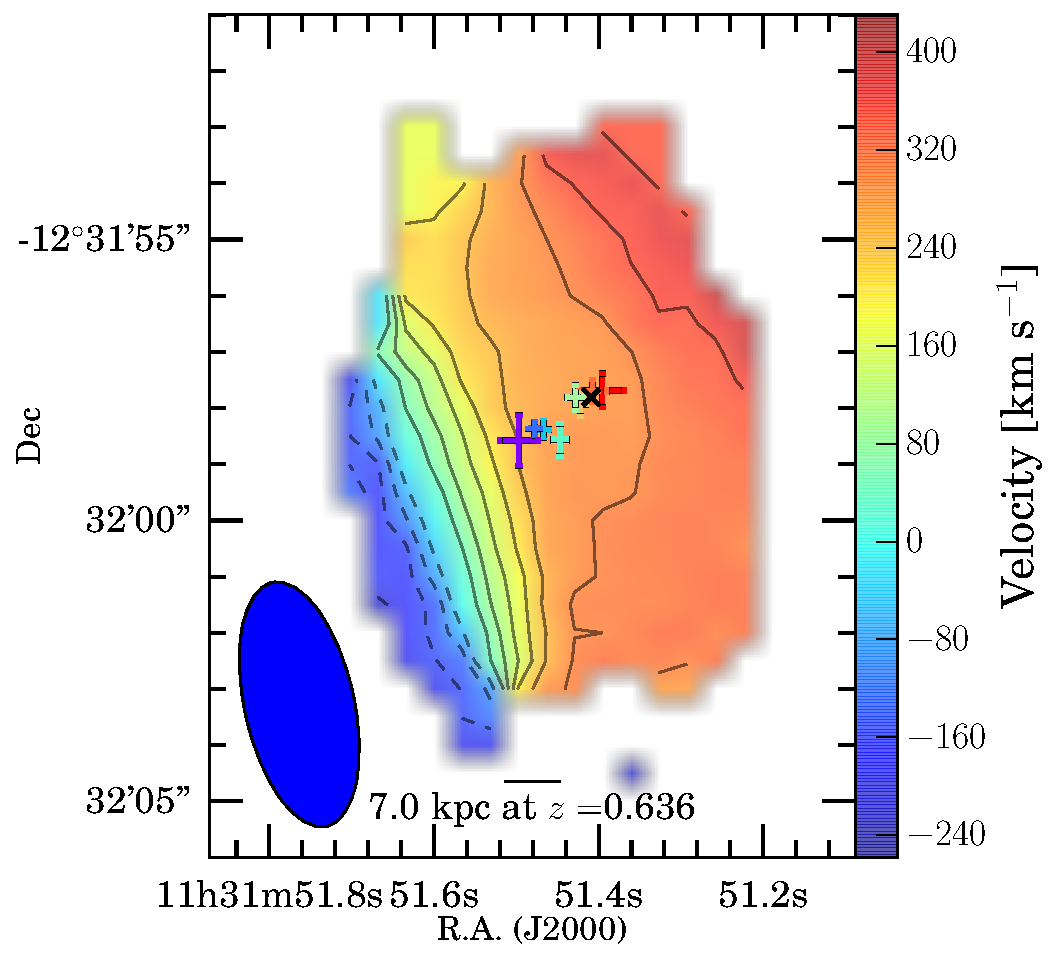
\includegraphics[width=0.4\textwidth]{../Figures/veloGradient_markers}
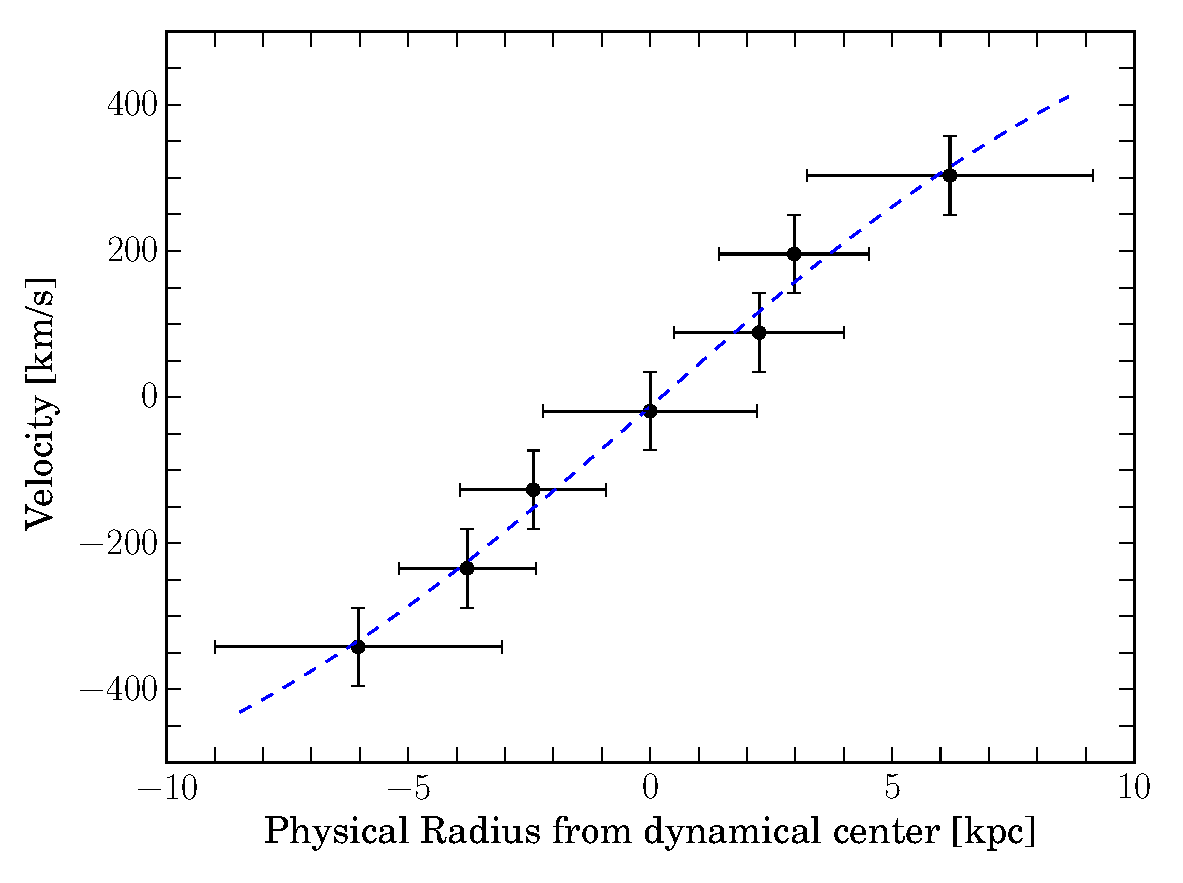
\includegraphics[width=0.455\textwidth]{../Figures/bestfit_PV.eps}
\caption{Top: Source-plane positions from best-fit \bco lens models are indicated with their associated uncertainties atop
the observed first moment map. The contours are at steps of 50\,\kms.
Bottom: PV slice along the major axis in the source plane at PA\,=\,121\degr.
Dashed line shows the best-fit rotation curve using an arctangent model.
The vertical error bars show the channel width for
each model and the horizontal error bars are the
1$\sigma$ uncertainties on the source plane positions.
 \label{fig:PV}}
\end{figure}

The asymptotic velocity ($V_{a}$) -- an extrapolation of the model
out to radius beyond the disk scale-length and half-light radius --
is not equivalent to maximum observed velocity ($V_{\rm max}$),
which is commonly used in literature to parameterize disc rotation.
The arctangent model is most commonly used in studies of the
Tully-Fisher relation, where an extrapolation to V$_{2.2}$ (velocity
at 2.2 disc scale-length or $\sim$1.375 half-light radius,
or $\sim$0.7$R_{\rm opt}$\footnote{Radius enclosing 83\% of the light
distribution.}) is typically adopted
as the rotation velocity ($V_{\rm max}$ in their
terminology) since this corresponds to the radius at which the velocity
of a pure exponential disc peaks.
We here adopt the maximum {\em observed} velocity
$V_{\rm rot}$\,=\,345\,$\pm$\,55\,\kms at 6\,$\pm$\,3\,kpc from the
dynamical center as a proxy to the rotation velocity.
This radius corresponds to $\sim$0.6$R_e$, where $R_e$ is the half-light
radius $\sim$10.3\,kpc inferred from the {\it HST} $I$-band
lens model (C06; converted to
our cosmology).
We note that the source plane half-light radius varies substantially with
wavelength. In particular, the half-light radius is found to be
$\sim$\,4kpc and $\sim$7\,kpc in $V$-band
\citep{Brewer08a} and $H$-band (C06), respectively.
This discrepancy arises owing to the exclusion of the more
diffused emission in $V$-band (rest-frame UV),
which traces young massive stars.
The $V$-band compactness may be explained in part
due to the fact that its emission is
more susceptible to dust extinction than other bands.
On the other hand, the molecular gas (fuel for \SF) is more compact
than the more evolved stellar population, as traced by $I$ and $H$-bands.
This is consistent with the picture that stars diffuse outward
after their formation \citep{Calzetti01a}.

Using our estimate of $V_{\rm rot}$, we find a dynamical mass of
$M_{\rm dyn}$\,sin$^2 i$\,($<$\,6\,kpc$)$\,=\,17\E{10}\,\Msun enclosed
within the CO-emitting region. If we instead consider the
line peak separation from the
\bco line profile $\Delta v_{\rm sep}/2 \sim$200\,\kms, we find
$M_{\rm dyn}$\,sin$^2 i$\,($<$\,6\,kpc$)$\,=\,5.8\E{10}\,\Msun.
We correct for the inclination effect using the
morphological axial ratio from the reconstructed image (Figure 3 in C06), where
the minor axis is 1\farcs8 and the major axis is 3\farcs25.
We thus find an inclination angle of 56.4\degr, which is consistent with the
observed unobscured AGN and an observable double peak line profile.
The dynamical mass is then
8.3\E{10}\Msun\,$<$\,$M_{\rm dyn}$($<$6\,kpc)\,$<$\,25\E{10}\Msun.
Since this quantity is derived under the assumption that the gas is
virialized, which is highly unlikely given the velocity dispersion and the
presence of a close companion, our estimate is
at most a lower limit.

\subsection{SED modeling} \label{sec:SED}  % DONE
We fit dust SED models to the
24\,\micron$-$2.2\,mm photometry in \Fig{SED}, where we also
include the IRAS 60\,$\micron$ and 100\,$\micron$ upper limits
to constrain the dust peak.
The fit is performed with the code
\ncode{mbb\_emcee} \citep[\eg][]{Riechers13a,Dowell14a}, which samples the posterior
using an MCMC approach and uses instrumental
response curves to perform color correction on-the-fly.
The SED model consists of a modified-blackbody
function with a power-law attached to the
Wien side to account for an excess in the MIR owing to warm,
small dust emission.
% Previous studies find that in the absence of mid-IR data, a powerlaw slope
% of $\alpha$ = 2 is consistent with SB and slightly more shallow, $\sim$1.5, % for SB/AGN composite systems (Blain et al., 2003; Casey, 2012; Koss et al., 2013).
%
%We add $\sim$15\% calibration uncertainties in quadrature to obtain the total
%uncertainties for the PdBI continuum in our fitting procedure.
The model is thus described by five free parameters: the rest-frame characteristic dust
temperature (T$_{d}$), the emissivity index ($\beta$), the power-law index
($\alpha$), the flux normalization at 500\,$\micron$ ($f_{\rm norm}$), and
the observed-frame wavelength at which the emission
becomes optically thick ($\lambda_{0}$). We impose
an upper limit of 100\,K on $T_d$, a Gaussian prior centered around
$\mu$\,=\,1.9 with $\sigma$\,=\,0.3 on $\beta$, and an upper limit of
1000\,$\micron$ on $\lambda_0$.
We check for chain convergence by requiring the autocorrelation
length of each parameter to be less than the number of steps
taken for the burn-in phase (which are then discarded).
Here we report the means % modes in log file
% summary statistics (global mode (where min. chi),
% marginal mode (in log file), posterior median (instead of posterior means;
% need to compute)
and the 1$\sigma$ confidence interval in the marginal PDFs
as the best-fit parameters, as listed in \Tab{SED}.

\begin{deluxetable}{lccc}[!htbp]
\tabletypesize{\scriptsize}
\tablecolumns{4}
\tablecaption{SED fitting results}
\tablehead{
\multicolumn{2}{c}{Parameters}      &
\colhead{With 24\micron} &
\colhead{Without 24\micron}
}
\startdata
$T_d$                           & (K)                & 52.0\petm{4.0}{4.1}   & 58.2\petm{14.5}{14.4}  \\ [1.05ex]
$\beta$                         &                    & 1.8\petm{0.5}{0.6}    & 2.1\petm{0.3}{0.3}  \\ [1.05ex]
$\alpha$                        &                    & 1.6\petm{0.5}{0.5}    & 8.9\petm{6.9}{6.3}   \\ [1.05ex]
$\lambda_0$\tna                 & ($\micron$)        & 548\petm{285}{307}    & 367\petm{125}{145}  \\ [1.05ex]
$\lambda_{\rm peak}$\tnb        & ($\micron$)        & 162\petm{16}{30}      & 146\petm{39}{44}  \\ [1.05ex]
$f_{\rm norm,\ 500\micron}$\tnc & (mJy)              & 59\petm{14}{13} & 60\petm{5}{5} \\ [1.05ex]
\LFIR\tnd                       & (10$^{12}$\,\Lsun) & 3.81\petm{2.04}{1.92} & 4.72\petm{2.54}{2.26}      \\ [1.05ex]
$M_{\rm d}$\tne                 & (10$^8$\,\Msun)    & 22\petm{5}{18}        & 11\petm{5}{6}
\enddata
\label{tab:SED}
\tablenotetext{a}{Observed-frame wavelength where $\tau_\nu$\,=\,1}
\tablenotetext{b}{Observed-frame wavelength of the SED peak}
\tablenotetext{c}{Observed-frame flux density at 500 $\micron$}
\tablenotetext{d}{Rest-frame 42.5$-$122.5\,$\micron$ luminosity}
\tablenotetext{e}{Derived assuming absorption mass coefficient of $\kappa$\eq2.64\,m$^2$\,kg$^{-1}$ at $\lambda$\,=\,125.0\,$\micron$ \citep{Dunne03a}}
\tablecomments{Errors reported here are $\pm$1$\sigma$.
\LFIR and $M_{\rm d}$ are not corrected for lensing.}
\end{deluxetable}



In the first model, we include the 24\,$\micron$ data
to constrain the power-law index. Based on the
best-fit of this model, we find a
\fir luminosity (rest-frame 42.5\,$-$\,122.5\,$\micron$) of
3.81\petm{2.04}{1.92}\E{12}\,\Lsun and a
dust mass of 22\petm{5}{18}\E{8}\,\Msun, uncorrected for lensing.
For the mass absorption coefficient, we adopt
$\kappa$\,=\,2.64\,m$^2$kg\pmOne at 125.0\,$\micron$
(rest frame; \citealt{Dunne03a}).
The dust mass uncertainty does not
include those in the absorption coefficient.

A fit including the MIR 24\,$\micron$ photometry
is likely an upper limit on the \fir luminosity arising from the starburst
in the AGN host galaxy.
% since the fit include contribution from the AGN (through power-law to MIR)
If we instead fit for a model excluding the 24\,$\micron$ constraint,
two major consequences are immediately apparent.
First, the power-law index is poorly-constrained (see \Tab{SED}).
Second, the steep power-law implies a small contribution
from the power-law regime
to the total IR luminosity as compared to the graybody.
Thus, the \fir luminosity in
this model should, in principle, corresponds to a
lower limit on the cold dust emission.
Using the best-fit parameters
for this model, we find a total IR luminosity
\LIR (rest-frame 8\,$-$\,1000\,\micron) of 8.14\petm{2.64}{2.80}\E{12}\,\Lsun,
a \fir luminosity \LFIR of 4.72\petm{2.54}{2.26}\E{12}\,\Lsun and a
dust mass $M_{\rm dust}$ of 11\petm{5}{6}\E{8}\,\Msun.
Taken at face value, this implies a \LFIR-to-\LIR ratio
of $\sim$58\pmm BLAH\%.
Again, the inferred quantities are uncorrected for lensing.
%The best-fit SEDs are shown in \Fig{SED} and the
% resulting parameters are listed in \Tab{SED}.

The dust temperature from both models is similar to that of
ULIRGs at 0.6\,$<$\,$z$\,$<$\,1.0 (54\,$\pm$\,5\,K; \citealt[hereafter C13]{Combes13a}).
We note the \fir luminosity is comparable in both models, which is
not surprising given the lack of constraints in the MIR. In fact, the
\fir luminosity from the second model is slightly higher than the former, but
consistent within the uncertainties.
For the subsequent analysis, we adopt the physical quantities
from the former (\ie with constraints at 24\,\micron).
The choice of SED model does not affect
the derived star formation rate (SFR) given the similar \fir luminosity.
Yet, the dust mass is higher in the former (but consistent within the
uncertainties), and thus the gas-to-dust ratio in \Sec{properties}
should be considered as an estimate.
We correct for lensing using the median magnification
factor $(\mu_{\rm L}\eq5.5)$
from the CO lens models. This yields a \LFIR of $($6.9\pmm3.6$)$\E{11}\,\Lsun.
Assuming a Salpeter initial
mass function \citep{Salpeter55a}, we find a
SFR of (120\pmm63)\,\Msun\,yr\pmOne using the
standard conversion \citep{Kennicutt98a}.

\begin{figure}[!htbp]
\centering
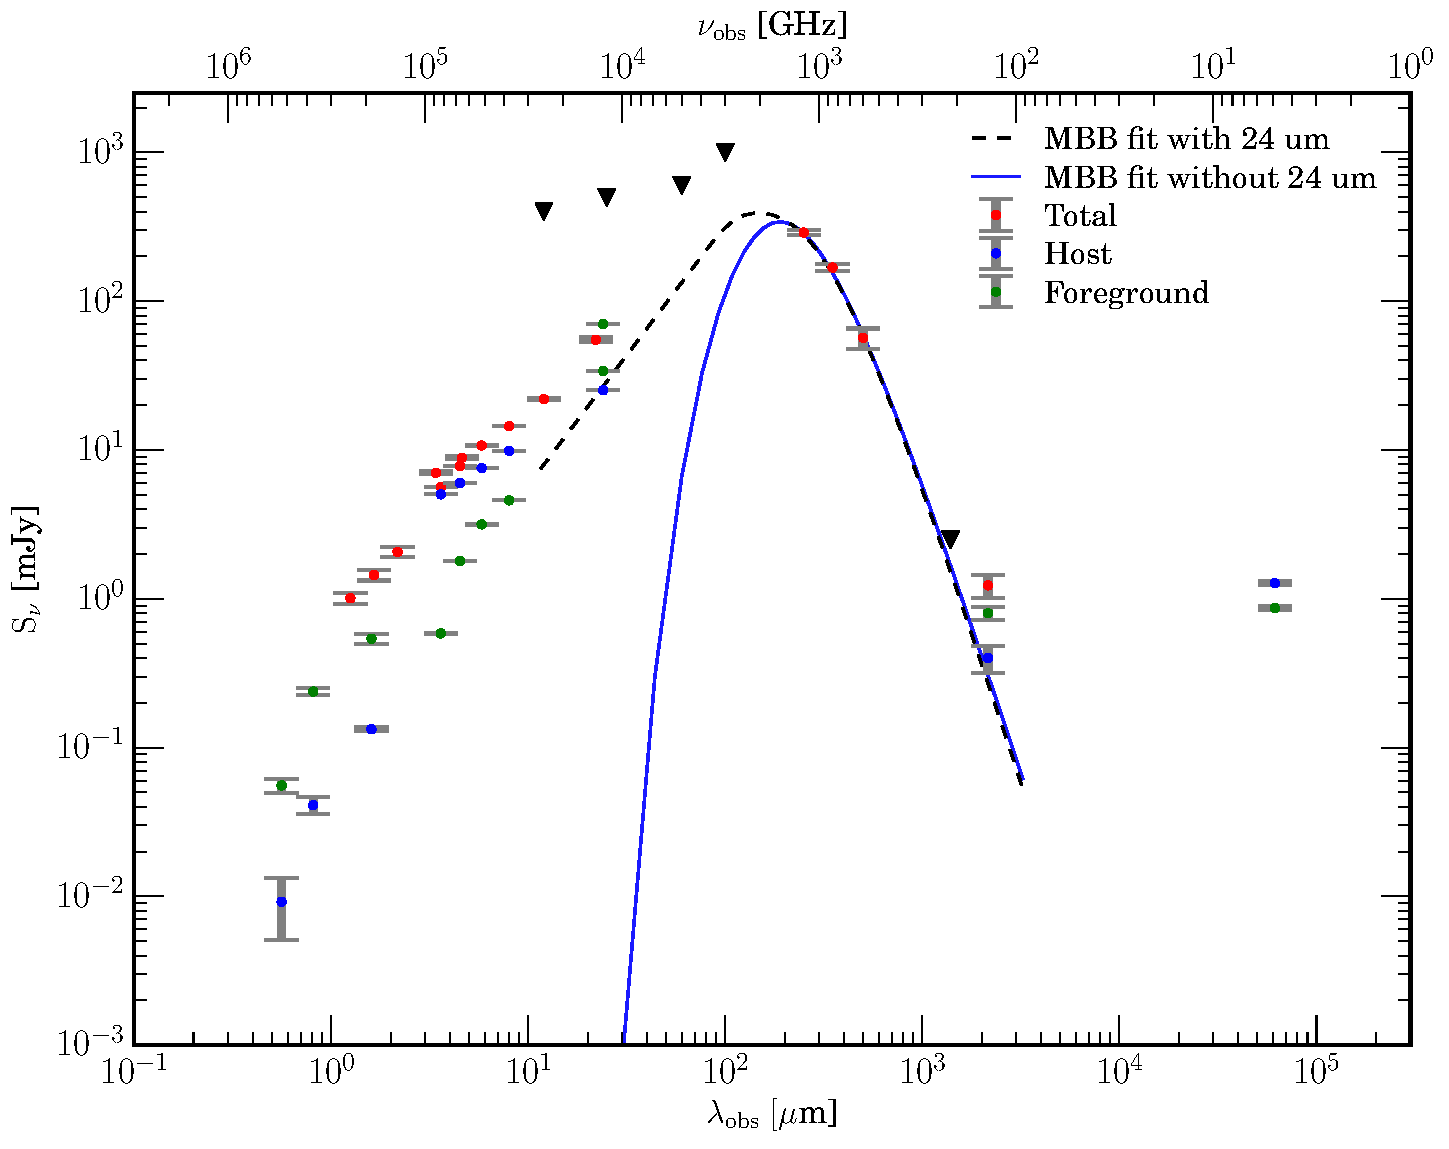
\includegraphics[trim=65 15 15 95, clip, width=0.45\textwidth]{../Figures/FullSED.eps}
\caption{SED models of the IR dust emission toward RXJ1131.
{\bf This figure needs an update}
WISE flux is slightly higher than the IRAC point, probably due to a smaller
aperture used in IRAC extraction,
both of which were taken from the archive.
IRAC: Aperture flux in 5\farcs diameter.
MIPS: use PSF fit flux from archive as source size $<$ PSF FWHM of 6$^{\prime\prime}$.
Might want to add NVSS constraints.
\label{fig:SED}}
\end{figure}


To place RXJ1131 in context of existing studies,
we compare its properties
with those reported by C13, which is the largest sample of
IR-luminous galaxy at similar redshift
(0.6\,$<$\,$z$\,$<$\,1.0) with CO measurements.
Since C13 adopt a different definition of
\LFIR (40\,$-$\,500\,\micron)\footnote{We also note that the
\fir luminosity in C13 is derived based on 60\,$\micron$ and 100\,$\micron$ IRAS fluxes.},
we derive the \fir luminosity following this convention.
This yields $($8.8\pmm0.4$)$\E{11}$(\mu_{\rm L}$/5.5$)\pmOne$\,\Lsun and
a SFR of $($150\pmm 70$)$\,\sfrU.
This implies that RXJ1131 is considered a LIRG in regard to their
sample, and consequently, the SFR of RXJ1131 is lower
(cf. SFR\,$>$\,200, with an average of 1200 in C13).
If we instead adopt the
more generally used definition for the total IR luminosity,
calculated using 8\,$-$\,1000\,\micron, RXJ1131 would be
considered a ULIRG given its lensing-corrected
total IR luminosity of $\sim$2\E{12}\,\Lsun.

\subsection{Gas properties} \label{sec:properties}
In this section, we derive the gas properties of RXJ1131 based on \bco,
and compare the derived quantities against those reported by
C13, where their results are based on \bco and \rot{4}{3} line observations on the IRAM 30-m dish.

\subsubsection{Linewidth \& Sizes} %DONE
We find that the linewidths for both components (redshifted and blueshifted)
inferred from a double Gaussian fit to the line profile are
comparable to the C13 ULIRG sample
($\Delta v_{\rm FWHM}$ of 370\,\kms) and local ULIRGs
(300\pmm85\,\kms; \citealt[][]{Solomon97a}).
Since C13 do not have resolved observations, we compare the
gas distribution with local U/LIRGs. The CO gas in RXJ1131 is
distributed $\sim$6\,kpc in radius across (in
the source plane), which is more extended than the
sample of disk-like U/LIRGs studied by
\citet[hereafter U14]{Ueda14a}, % also classified U/LIRG using FIR from 60, 100 micron measurements
who find an average radius of 3.5\,$\pm$\,2.3\,kpc
with a range spanning 1.1\,$-$\,9.3\,kpc.
% This is expected if the positive correlation in the linewidth-size relation
% holds at intermediate redshifts. Yet we cannot quantify this further
% with the data represented in this paper.

\subsubsection{Gas Mass}
To derive the molecular gas mass, we first correct for lensing magnification
using the respective magnification factors listed in \Tab{model}, which to
first order takes into account effect of differential lensing. This yields
$I_{\small \bco}$\,=\,5.9$\pm$2.7 Jy\,\kms,
where the uncertainty includes those on
the magnification factors.
We note that this includes emission from the companion
as the spatial resolution of our data do not allow us decompose its
contribution from the total line flux.

Without direct \rot{1}{0} measurements,
we derive \rot{1}{0} intensity
using a brightness temperature ratio of $r_{\rm 32}$\,=\,1, which was chosen
solely to facilitate a comparison with other U/LIRGs.
For the same reason, we
adopt a luminosity-to-mass conversion factor of
\alphaco\,=\,0.8 (K \kms pc$^2$)\pmOne, this yields a
CO luminosity \Lp\,=\,(3.47\,$\pm$\,1.58)\E{10}\,\LpU and a gas mass
$M_{\rm gas}$ of (2.8$\pm$1.3)\,\E{10} \Msun. This is likely
an overestimation for RXJ1131 due to a contribution from the companion.
The inferred gas mass is comparable to
C13 sample ($M_{\rm gas}$\,=\,1.5\E{10}\Msun) as well as
local U/LIRGs \citep{Solomon97a, Sanders96a} but higher than
local LIRGs (U14).

% gas-to-dyn ratio
We place a lower limit on the dynamical mass (see \Sec{dynamics}) using
the inferred gas mass. This BLAH.
 {\bf will need edit depending on the dyn. modeling section}
a gas-to-dynamical mass fraction of $f_{\rm gas-dyn}$\,=\,BLAH.
% gas to dust ratio:
Using the dust mass derived from SED fitting,
we find a gas-to-dust ratio of 184\pmm124, which is consistent with
the C13 sample ($f_{\rm gas-dust}$\,=\,206) and local U/LIRGs
(200$-$350; \citealt{Sanders91a}, Contini \& Contini 2003; Seaquist et al. 2004; Wilson et al. 2008).

\subsubsection{SFE and Depletion Time}
We derive the SFE using the far-IR luminosity definition used by
C13 (\ie SFE\pmm\LFIR$($40\,$-$\,500\,\micron)$/$$M_{\rm gas}$$)$,
we find a SFE of 31\pmm15 for RXJ1131, or equivalently a depletion
timescale of $\tau$\,=\,190\pmm70\,Myr. % 5.8/SFE Gyr
This SFE is substantially lower than most U/LIRGs
(\citealt{Solomon97a,Combes11a}; C13). % local ULIRG: 180 +/- 160 Lsun/M (Solomon+97)
% Combes+13: sample of 39 gal from z= 0.2-1 find $<$ 100 Myr.

Implication of this unexpectedly low SFE in RXJ1131...




%--------------------------------------------------------------------------
%                                Discussion
%--------------------------------------------------------------------------
\section{Discussion} \label{sec:diss}
\subsection{Merger stage of RXJ1131-1231}
In this section, we put our results in context with other ULIRGs/mergers at
$z$\,=\,0\,$-$\,1. It is clear that RXJ1131 has a
gas-rich companion, but how does this affect its internal dynamics?
What is the merger stage of RXJ1131?
We argued that the symmetric source-plane velocity field suggest
the system is a minor merger, consistent with an earlier study by B08, who
independently conclude that the companion is likely
a dwarf of size $\sim$700\,kpc across.

While our result is consistent with other studies of RXJ1131, it
contrast strongly with studies of local (U)LIRGs/mergers
(\LIR\,=\,10$^{11-12.5}$\,\Lsun; $z$\,$<$\,0.1), where AGNs are
typically found in late stage mergers
\citep{Yuan10a,Iwasawa11a,Carpineti12a} and
that only these major mergers near their final
coalescence can provide \LIR\,$>$\,10$^{12}$\,\Lsun,
\citep[\eg][hereafter L16]{Carpineti15a,Larson16a}
\footnote{In this section, we adopt the total IR luminosity
calculated from 8\,$-$\,1000\,$\micron$
to be consistent with the classification used by these authors.}.
If this is also the case at $z$$\sim$0.65, it would imply RXJ1131
is a major merger near its final coalescence and that the spatially offset
component is likely an expulsion of gas driven by AGN winds or some
tidally ejected material from previous passage.
In that case, the molecular gas fraction in the host
galaxy should have declined (as seen in ellipticals) compared to early
stage mergers
\textbf{can we find molecular gas mass fraction as a
function of merger stage? also, what is the dynamical mass for RXJ1131}
and that the molecular gas would
be more concentrated in the nuclear region.
This is inconsistent with what
is observed for RXJ1131
(an extended gas-rich disk; but see also U14 for outliers
with extended molecular gas in merger remnants) and
the fact that there is on-going \SF activity.
Hence, we reject this and speculate the discrepancy is a consequence
of different power mechanisms of IR-luminous galaxies at intermediate redshift.

{\bf --- anything below is not ready ---}
\subsubsection{Fate of RXJ1131-1231}
Has RXJ1131 encountered with the companion?

From numerical simulations, mergers are observable and distinguishable
with their kinematic and morphological features for 0.2$-$0.4 Gyr
between their second passage and final coalescence.

The spinning black hole in RXJ1131 provide one piece of
evidence that the two has already encountered.


% The future of RXJ1131:
Mergers are expected to evolve into
local ellipticals or large-disks (bulge dominated) (springel \& Hernquist 05, cite).
Given the
extended molecular gas distribution, we suggest RXJ1131 may evolve into the
latter (large-disk) unless the ``companion'' BKAH SOME STUFF or some other
mechanisms at play in the latter stage, transporting the gas
toward the central nuclear region and blah.

\subsection{ULIRG Evolution and Cosmic SFH}
While there is an emerging consensus on the strong
evolution of the IR luminosity function \citep[\eg][]{Huynh07a,Seymour10a},
it is currently unclear whether the IR luminosity of
these intermediate redshift sources arise due to the merging of large spiral
galaxies, as typically seen in local ULIRGs, or proceed under a different
formation processes at higher redshifts. Our study blah...

% Implication on SFH
Our result indicates that...
% the gas mass fraction has already decreased
% at this redshift, which may suggest that the change in cosmic SFD is due to
% change in gas content. The SFE is also BLAH at this redshift,
% consistent with current speculation of how the SFRD decreases over cosmic time.

%--------------------------------------------------------------------------
%                                Conclusions
%--------------------------------------------------------------------------
\section{Summary and Conclusions} \label{sec:sum}
% see Hodge12_dynamics.pdf for guide

%- summarize the findings from the entire study
%    - firm conclusions
%    - speculative possibilities

We investigate the cold gas kinematics and dynamics in
the lensed optical quasar RXJ1131 at $z_{\rm CO}$\,$\sim$0.65
by observing its \bco and \cco line emission.
Our results suggest that RXJ1131 is a wet-wet merger between an AGN/starburst
ULIRG and a optically faint companion.

% Fitting SED models, we find that the AGN host galaxy is a ULIRG.
% A faint companion as seen in HST observations (BJB) is also detected in our CO, confirming it's redshift and gas rich nature.

% % any further work needed to resolve the remaining problems
% We list several pieces of evidence through out
% this work to argue that RXJ1131 is likely a rotating disk.
% The double-horned profile, smooth, symmetric velocity field
% seen in our lens model and in the
% image plane and C06 model $n$=1 Sersic profile all suggest
% a kinematically-order (i.e., disk) galaxy.
% Yet, these are insufficient to conclude a disk morphology. Additional
% characteristics such as peak velocity dispersion at the central region and a
% ``spider'' diagram are needed, which is commonly seen in local spirals.
% The high dispersion near the dynamical center also
% suggest that RXJ1131 is turbulent, albeit lack of spatial resolution. Overall
% implies RXJ1131 is a minor merger of a turbulent disc, but higher-resolution
% data are needed to confirm this.

%==============================================================================
%                                Back matters
%==============================================================================


% ACKNOWLEDGEMENTS
%-----------------
\acknowledgments
This work is based on observations carried out under project number S14BX001
with the IRAM NOEMA Interferometer. IRAM is supported by INSU/CNRS (France), MPG (Germany) and IGN (Spain).
Support for CARMA construction was derived from the Gordon and Betty Moore
Foundation, the Kenneth T. and Eileen L. Norris Foundation, the James S.
McDonnell Foundation, the Associates of the California Institute of
Technology, the University of Chicago, the states of Illinois, California, and
Maryland, and the National Science Foundation. Ongoing CARMA development and
operations are supported by the National Science Foundation under a
cooperative agreement and by the CARMA consortium universities.
The National Radio Astronomy Observatory is a facility of the National Science
Foundation operated under cooperative agreement by Associated
Universities, Inc.
This research made use of data obtained with {\it Herschel}, an ESA space
observatory with science instruments provided by European-led Principal
Investigator consortia and with important participation from NASA.
This research has made use of NASA's Astrophysics Data System Bibliographic
Services.
This work is based in part on observations made with the \spitzer,
which is operated by the Jet Propulsion Laboratory, California Institute of
Technology under a contract with NASA.
This publication made use of data products from the Wide-field Infrared
Survey Explorer, which is a joint project of the University of California, Los
Angeles, and the Jet Propulsion Laboratory/California Institute of Technology,
funded by the National Aeronautics and Space Administration.
This publication made use of data products from the Two Micron All Sky
Survey, which is a joint project of the University of Massachusetts and the
Infrared Processing and Analysis Center/California Institute of Technology,
funded by the National Aeronautics and Space Administration and the National
Science Foundation.
This research made use of the NASA/IPAC Extragalactic Database (NED) which
is operated by the Jet Propulsion Laboratory, California Institute of
Technology, under contract with the National Aeronautics and Space
Administration.
This research made use of Astropy, a community-developed core Python package for Astronomy \citep{astropy}.
This research made use of APLpy, an open-source plotting package for Python hosted at \url{http://aplpy.github.com}.

Facilities: IRAM PdBI, CARMA, VLA, Herschel (SPIRE), WISE, IRAS, 2MASS, Spitzer(IRAC, MIPS), HST(ACS, NICMOS)


  %--------------------------------------------------------------------------
  %                               Bibliography
  %--------------------------------------------------------------------------
\bibliographystyle{yahapj}
\bibliography{RXJ.bib}
\end{document}